\documentclass[8pt]{beamer}

% Beamer style
%\usetheme[secheader]{Madrid}
% \usetheme{CambridgeUS}
\useoutertheme{infolines}
\usecolortheme[rgb={0.65,0.15,0.25}]{structure}
% \usefonttheme[onlymath]{serif}
\beamertemplatenavigationsymbolsempty
%\AtBeginSubsection

% Packages
%\usepackage[french]{babel}
\usepackage[latin1]{inputenc}
\usepackage{color}
\usepackage{xspace}
\usepackage{dsfont, stmaryrd}
\usepackage{amsmath, amsfonts, amssymb, stmaryrd}
\usepackage{epsfig}
\usepackage{tikz}
\usepackage{url}
% \usepackage{ulem}
\usepackage{/home/robin/LATEX/Biblio/astats}
%\usepackage[all]{xy}
\usepackage{graphicx}
\usepackage{xspace}

% Maths
% \newtheorem{theorem}{Theorem}
% \newtheorem{definition}{Definition}
\newtheorem{proposition}{Proposition}
% \newtheorem{assumption}{Assumption}
% \newtheorem{algorithm}{Algorithm}
% \newtheorem{lemma}{Lemma}
% \newtheorem{remark}{Remark}
% \newtheorem{exercise}{Exercise}
% \newcommand{\propname}{Prop.}
% \newcommand{\proof}{\noindent{\sl Proof:}\quad}
% \newcommand{\eproof}{$\blacksquare$}

% \setcounter{secnumdepth}{3}
% \setcounter{tocdepth}{3}
\newcommand{\pref}[1]{\ref{#1} p.\pageref{#1}}
\newcommand{\qref}[1]{\eqref{#1} p.\pageref{#1}}

% Colors : http://latexcolor.com/
\definecolor{darkred}{rgb}{0.65,0.15,0.25}
\definecolor{darkgreen}{rgb}{0,0.4,0}
\definecolor{darkred}{rgb}{0.65,0.15,0.25}
\definecolor{amethyst}{rgb}{0.6, 0.4, 0.8}
\definecolor{asparagus}{rgb}{0.53, 0.66, 0.42}
\definecolor{applegreen}{rgb}{0.55, 0.71, 0.0}
\definecolor{awesome}{rgb}{1.0, 0.13, 0.32}
\definecolor{blue-green}{rgb}{0.0, 0.87, 0.87}
\definecolor{red-ggplot}{rgb}{0.52, 0.25, 0.23}
\definecolor{green-ggplot}{rgb}{0.42, 0.58, 0.00}
\definecolor{purple-ggplot}{rgb}{0.34, 0.21, 0.44}
\definecolor{blue-ggplot}{rgb}{0.00, 0.49, 0.51}

% Commands
\newcommand{\backupbegin}{
   \newcounter{finalframe}
   \setcounter{finalframe}{\value{framenumber}}
}
\newcommand{\backupend}{
   \setcounter{framenumber}{\value{finalframe}}
}
\newcommand{\emphase}[1]{\textcolor{darkred}{#1}}
\newcommand{\comment}[1]{\textcolor{gray}{#1}}
\newcommand{\paragraph}[1]{\textcolor{darkred}{#1}}
\newcommand{\refer}[1]{{\small{\textcolor{gray}{{\cite{#1}}}}}}
\newcommand{\Refer}[1]{{\small{\textcolor{gray}{{[#1]}}}}}
\newcommand{\goto}[1]{{\small{\textcolor{blue}{[\#\ref{#1}]}}}}
\renewcommand{\newblock}{}

\newcommand{\tabequation}[1]{{\medskip \centerline{#1} \medskip}}
% \renewcommand{\binom}[2]{{\left(\begin{array}{c} #1 \\ #2 \end{array}\right)}}

% Variables 
\newcommand{\Abf}{{\bf A}}
\newcommand{\Beta}{\text{B}}
\newcommand{\Bcal}{\mathcal{B}}
\newcommand{\Bias}{\xspace\mathbb B}
\newcommand{\Cor}{{\mathbb C}\text{or}}
\newcommand{\Cov}{{\mathbb C}\text{ov}}
\newcommand{\cl}{\text{\it c}\ell}
\newcommand{\Ccal}{\mathcal{C}}
\newcommand{\cst}{\text{cst}}
\newcommand{\Dcal}{\mathcal{D}}
\newcommand{\Ecal}{\mathcal{E}}
\newcommand{\Esp}{\xspace\mathbb E}
\newcommand{\Espt}{\widetilde{\Esp}}
\newcommand{\Covt}{\widetilde{\Cov}}
\newcommand{\Ibb}{\mathbb I}
\newcommand{\Fcal}{\mathcal{F}}
\newcommand{\Gcal}{\mathcal{G}}
\newcommand{\Gam}{\mathcal{G}\text{am}}
\newcommand{\Hcal}{\mathcal{H}}
\newcommand{\Jcal}{\mathcal{J}}
\newcommand{\Lcal}{\mathcal{L}}
\newcommand{\Mt}{\widetilde{M}}
\newcommand{\mt}{\widetilde{m}}
\newcommand{\Nbb}{\mathbb{N}}
\newcommand{\Mcal}{\mathcal{M}}
\newcommand{\Ncal}{\mathcal{N}}
\newcommand{\Ocal}{\mathcal{O}}
\newcommand{\pt}{\widetilde{p}}
\newcommand{\Pt}{\widetilde{P}}
\newcommand{\Pbb}{\mathbb{P}}
\newcommand{\Pcal}{\mathcal{P}}
\newcommand{\Qcal}{\mathcal{Q}}
\newcommand{\qt}{\widetilde{q}}
\newcommand{\Rbb}{\mathbb{R}}
\newcommand{\Sbb}{\mathbb{S}}
\newcommand{\Scal}{\mathcal{S}}
\newcommand{\st}{\widetilde{s}}
\newcommand{\St}{\widetilde{S}}
\newcommand{\Tcal}{\mathcal{T}}
\newcommand{\todo}{\textcolor{red}{TO DO}}
\newcommand{\Ucal}{\mathcal{U}}
\newcommand{\Un}{\math{1}}
\newcommand{\Vcal}{\mathcal{V}}
\newcommand{\Var}{\mathbb V}
\newcommand{\Vart}{\widetilde{\Var}}
\newcommand{\Zcal}{\mathcal{Z}}

% Symboles & notations
\newcommand\independent{\protect\mathpalette{\protect\independenT}{\perp}}\def\independenT#1#2{\mathrel{\rlap{$#1#2$}\mkern2mu{#1#2}}} 
\renewcommand{\d}{\text{\xspace d}}
\newcommand{\gv}{\mid}
\newcommand{\ggv}{\, \| \, }
% \newcommand{\diag}{\text{diag}}
\newcommand{\card}[1]{\text{card}\left(#1\right)}
\newcommand{\trace}[1]{\text{tr}\left(#1\right)}
\newcommand{\matr}[1]{\boldsymbol{#1}}
\newcommand{\matrbf}[1]{\mathbf{#1}}
\newcommand{\vect}[1]{\matr{#1}} %% un peu inutile
\newcommand{\vectbf}[1]{\matrbf{#1}} %% un peu inutile
\newcommand{\trans}{\intercal}
\newcommand{\transpose}[1]{\matr{#1}^\trans}
\newcommand{\crossprod}[2]{\transpose{#1} \matr{#2}}
\newcommand{\tcrossprod}[2]{\matr{#1} \transpose{#2}}
\newcommand{\matprod}[2]{\matr{#1} \matr{#2}}
\DeclareMathOperator*{\argmin}{arg\,min}
\DeclareMathOperator*{\argmax}{arg\,max}
\DeclareMathOperator{\sign}{sign}
\DeclareMathOperator{\tr}{tr}
\newcommand{\ra}{\emphase{$\rightarrow$} \xspace}

% Hadamard, Kronecker and vec operators
\DeclareMathOperator{\Diag}{Diag} % matrix diagonal
\DeclareMathOperator{\diag}{diag} % vector diagonal
\DeclareMathOperator{\mtov}{vec} % matrix to vector
\newcommand{\kro}{\otimes} % Kronecker product
\newcommand{\had}{\odot}   % Hadamard product

% TikZ
\newcommand{\nodesize}{2em}
\newcommand{\edgeunit}{2.5*\nodesize}
\newcommand{\edgewidth}{1pt}
\tikzstyle{node}=[draw, circle, fill=black, minimum width=.75\nodesize, inner sep=0]
\tikzstyle{square}=[rectangle, draw]
\tikzstyle{param}=[draw, rectangle, fill=gray!50, minimum width=\nodesize, minimum height=\nodesize, inner sep=0]
\tikzstyle{hidden}=[draw, circle, fill=gray!50, minimum width=\nodesize, inner sep=0]
\tikzstyle{hiddenred}=[draw, circle, color=red, fill=gray!50, minimum width=\nodesize, inner sep=0]
\tikzstyle{observed}=[draw, circle, minimum width=\nodesize, inner sep=0]
\tikzstyle{observedred}=[draw, circle, minimum width=\nodesize, color=red, inner sep=0]
\tikzstyle{eliminated}=[draw, circle, minimum width=\nodesize, color=gray!50, inner sep=0]
\tikzstyle{empty}=[draw, circle, minimum width=\nodesize, color=white, inner sep=0]
\tikzstyle{blank}=[color=white]
\tikzstyle{nocircle}=[minimum width=\nodesize, inner sep=0]

\tikzstyle{edge}=[-, line width=\edgewidth]
\tikzstyle{edgebendleft}=[-, >=latex, line width=\edgewidth, bend left]
\tikzstyle{edgebendright}=[-, >=latex, line width=\edgewidth, bend right]
\tikzstyle{lightedge}=[-, line width=\edgewidth, color=gray!50]
\tikzstyle{lightedgebendleft}=[-, >=latex, line width=\edgewidth, bend left, color=gray!50]
\tikzstyle{lightedgebendright}=[-, >=latex, line width=\edgewidth, bend right, color=gray!50]
\tikzstyle{edgered}=[-, line width=\edgewidth, color=red]
\tikzstyle{edgebendleftred}=[-, >=latex, line width=\edgewidth, bend left, color=red]
\tikzstyle{edgebendrightred}=[-, >=latex, line width=\edgewidth, bend right, color=red]

\tikzstyle{arrow}=[->, >=latex, line width=\edgewidth]
\tikzstyle{arrowbendleft}=[->, >=latex, line width=\edgewidth, bend left]
\tikzstyle{arrowbendright}=[->, >=latex, line width=\edgewidth, bend right]
\tikzstyle{arrowred}=[->, >=latex, line width=\edgewidth, color=red]
\tikzstyle{arrowbendleftred}=[->, >=latex, line width=\edgewidth, bend left, color=red]
\tikzstyle{arrowbendrightred}=[->, >=latex, line width=\edgewidth, bend right, color=red]
\tikzstyle{arrowblue}=[->, >=latex, line width=\edgewidth, color=blue]
\tikzstyle{dashedarrow}=[->, >=latex, dashed, line width=\edgewidth]
\tikzstyle{dashededge}=[-, >=latex, dashed, line width=\edgewidth]
\tikzstyle{dashededgebendleft}=[-, >=latex, dashed, line width=\edgewidth, bend left]
\tikzstyle{lightarrow}=[->, >=latex, line width=\edgewidth, color=gray!50]

\newcommand{\CTSBM}{{\sl ct}-SBM\xspace}
\newcommand{\DTSBM}{{\sl dt}-SBM\xspace}

% Directory
\newcommand{\fignet}{/home/robin/Bureau/RECHERCHE/RESEAUX/EXPOSES/FIGURES}
\newcommand{\figeco}{/home/robin/Bureau/RECHERCHE/ECOLOGIE/EXPOSES/FIGURES}
% \newcommand{\figchp}{/home/robin/Bureau/RECHERCHE/RUPTURES/EXPOSES/FIGURES}
% \newcommand{\figfig}{../figs}
\newcommand{\figCMR}{/home/robin/Bureau/RECHERCHE/ECOLOGIE/CountPCA/pln/Article/Network_JCGS/trunk/figs}
\newcommand{\figDoR}{/home/robin/Bureau/RECHERCHE/BAYES/VBEM-IS/VBEM-IS.git/Data/Tree/Fig}
\newcommand{\figbordeaux}{/home/robin/Bureau/RECHERCHE/EXPOSES/RESEAUX/1904-Bordeaux}

%====================================================================
%====================================================================
\setcounter{tocdepth}{1}
\AtBeginSection{%
\begin{frame}
  \frametitle{\inserttitle}
%   \framesubtitle{Outline}
  \tableofcontents[currentsection]
\end{frame}
}


%====================================================================
%====================================================================
\begin{document}
%====================================================================
%====================================================================

%====================================================================
\title[Statistical network analysis]{Statistical network analysis}

\author[S. Robin]{St�phane Robin}

\institute[Sorbonne Universit� / LPSM]{Sorbonne Universit� / Laboratoire de Probabilit�s, Statistique et Mod�lisation}

\date[(JC)2BIM'21, Dijon]{\'Ecole (JC)2BIM 2021, Rennes, D�c. 2021}

%====================================================================
%====================================================================
\maketitle
%====================================================================


%-------------------------------------------------------------------------------
%-------------------------------------------------------------------------------
\section*{Introduction}
%-------------------------------------------------------------------------------
%-------------------------------------------------------------------------------

%-------------------------------------------------------------------------------
%-------------------------------------------------------------------------------
\subsection*{Two main questions}
%-------------------------------------------------------------------------------

%------------------------------------------------------------------------------
\frame{ \frametitle{Network analysis}

  \paragraph{Networks} are convenient to describe interactions between a set of entities, i.e.
  \begin{itemize}
    \item genes within a cell, 
    \item microbes within a medium, 
    \item neurones in a brain, 
    \item \dots
  \end{itemize}
  
  $$
  \begin{tabular}{cc}
    \begin{tabular}{c}
      \includegraphics[width=.3\textwidth]{\fignet/im_EcoliBVEM}
    \end{tabular}
    & 
    \begin{tabular}{c}    
      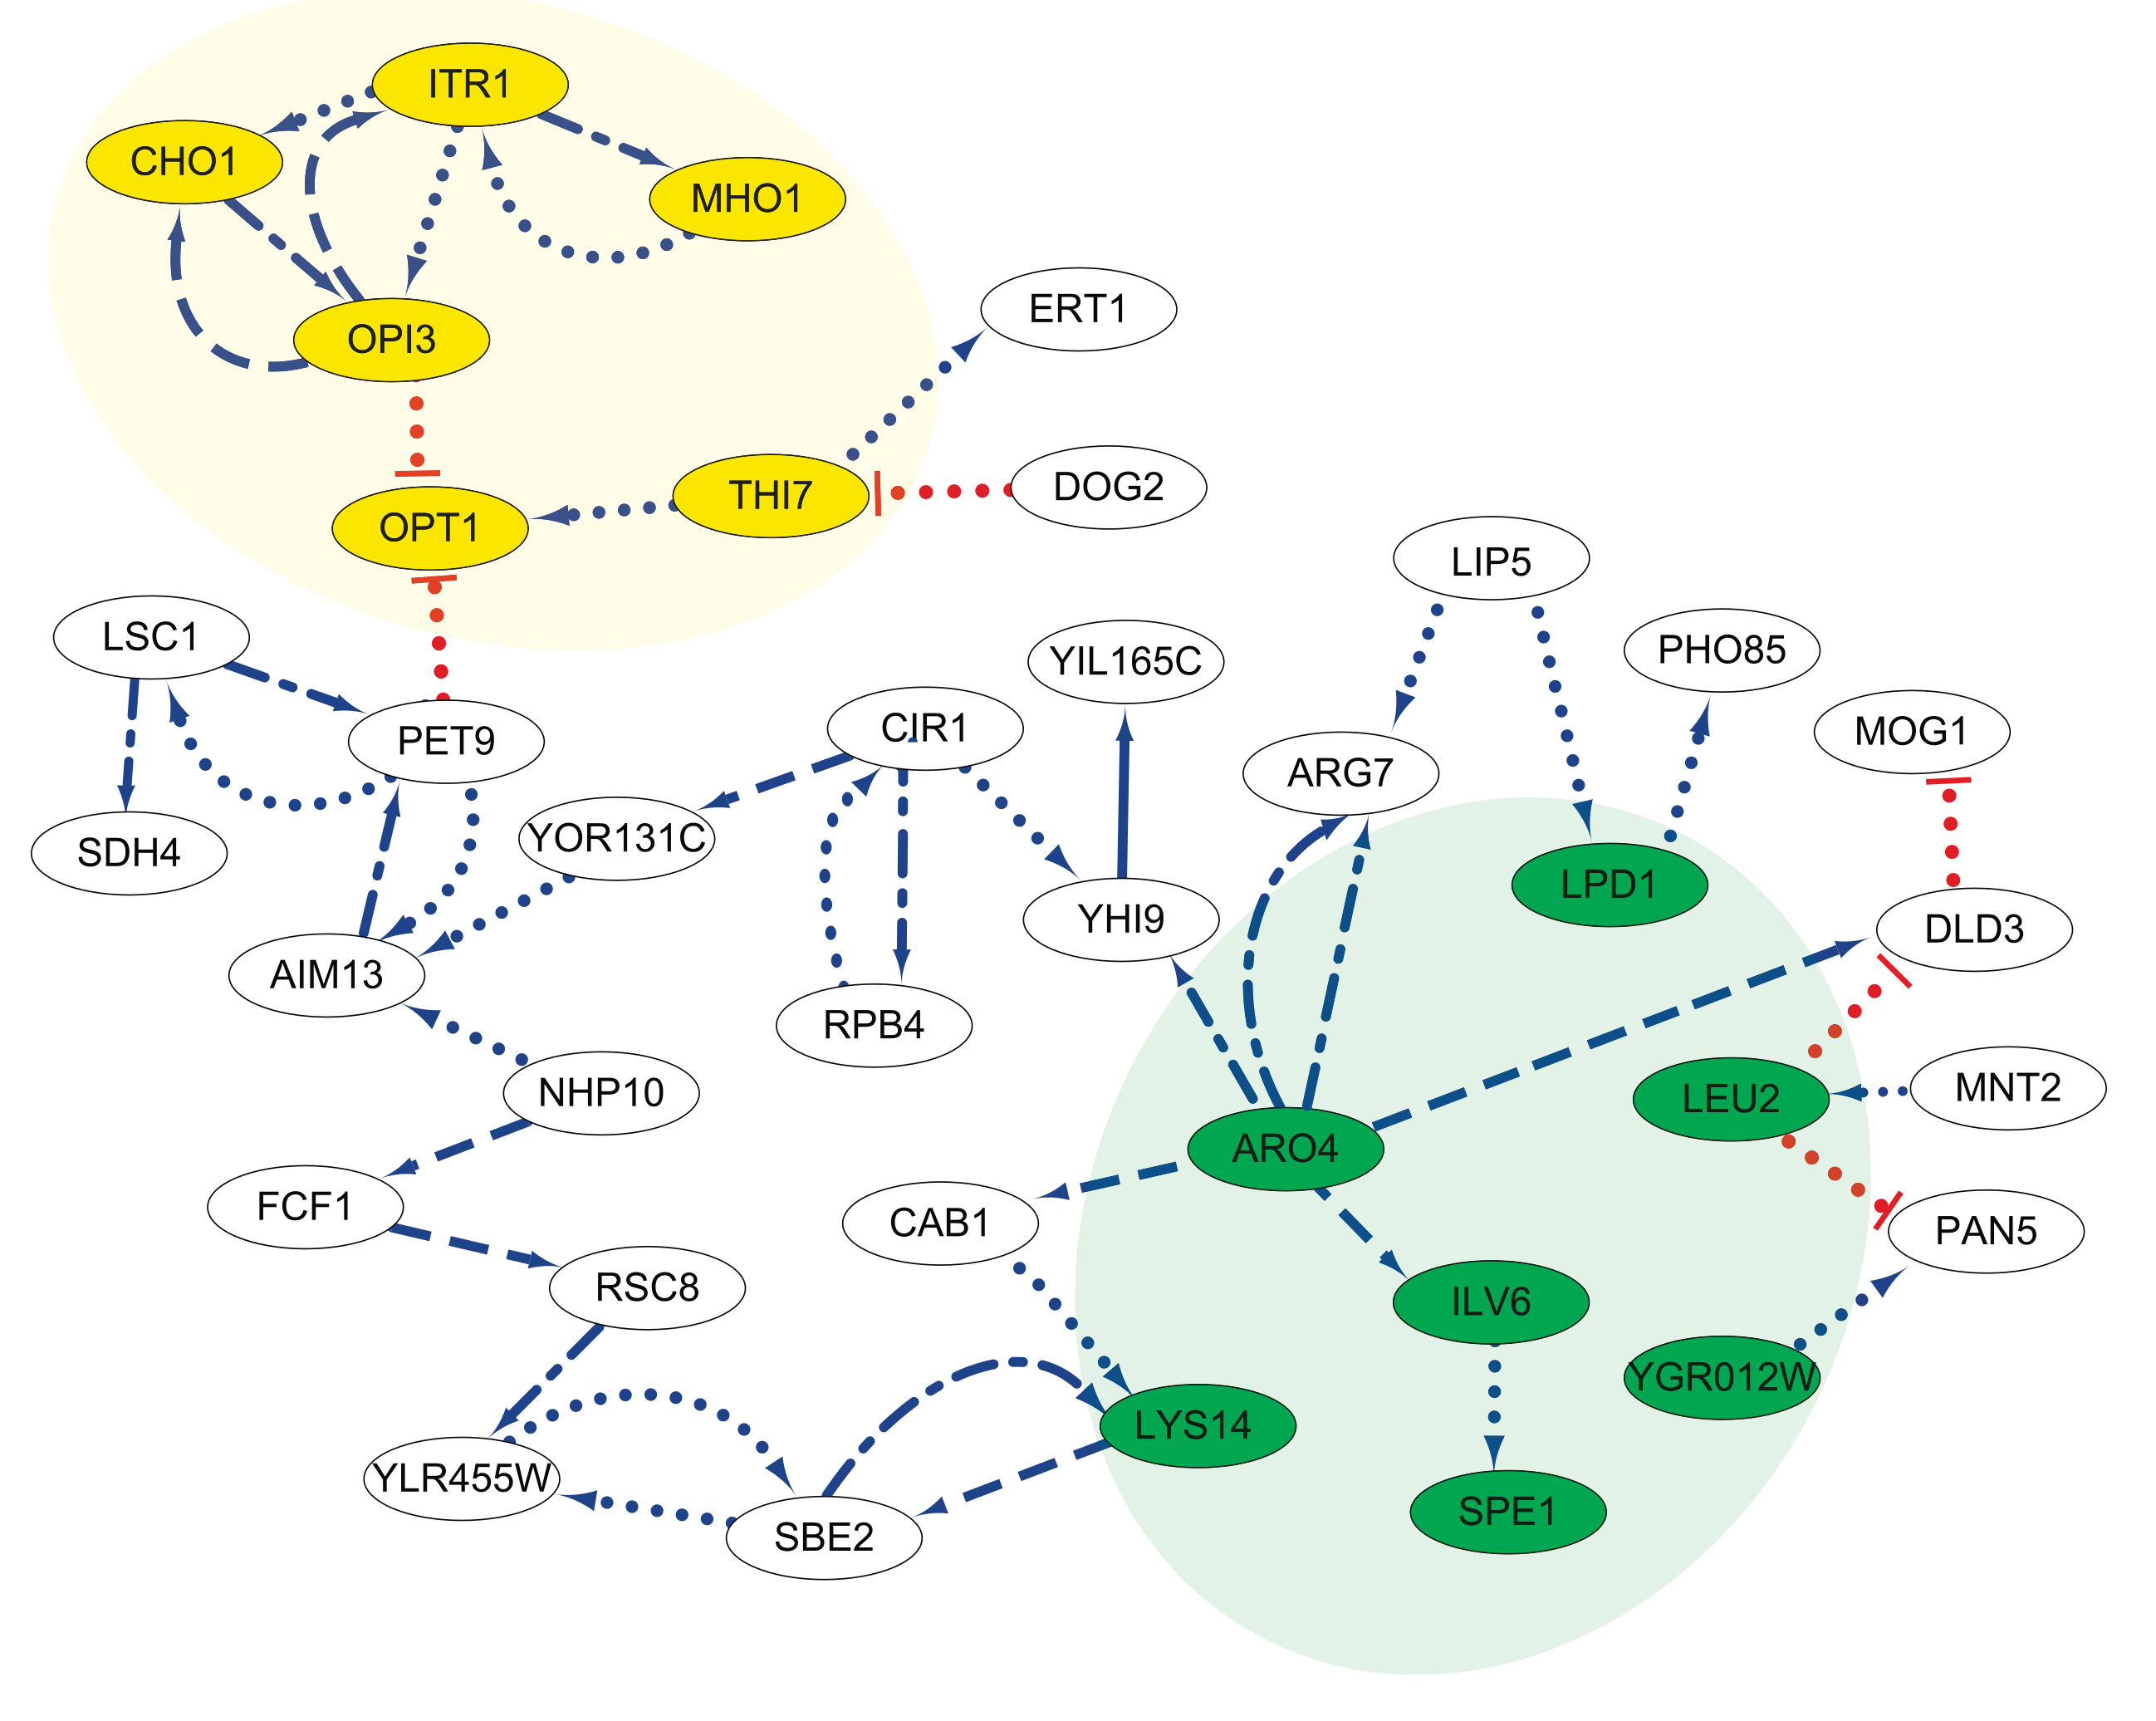
\includegraphics[width=.3\textwidth]{\fignet/CZH19-Nature-Fig1}
    \end{tabular}
  \end{tabular}
  $$
}

%------------------------------------------------------------------------------
\frame{ \frametitle{A bit of vocabulary}

  \paragraph{Definition.} 
  \begin{align*}
    \text{Network} & = \text{ biological object} \\
    \text{Graph} & = \text{ its mathematical representation} \\
  \end{align*}

  \bigskip \pause
  \paragraph{Correspondance.}
  $$
  \begin{tabular}{ccc}
    Network & & Graph $G = (V, E)$ \\
    \hline
    Entity (gene, microbe, neurone, \dots) & $=$ & Vertex (or node) \\
    'Interaction' & $=$ & Edge 
  \end{tabular}
  $$
  
  \bigskip \pause
  Depending on the type of interaction, edges can be 
  \begin{itemize}
   \item binary (presence/absence) or valued (weighted), 
   \item undirected or directed, 
   \item univariate or multivariate, 
   \item \dots
  \end{itemize}
  
}

%------------------------------------------------------------------------------
\frame{ \frametitle{Observed network}

  \begin{tabular}{cc}
    \hspace{-.04\textwidth}
    \begin{tabular}{p{.5\textwidth}}
        \paragraph{Observed network.} \\
        'Interaction' between each pair of entities have been observed or tested, in a experimental manner (think of protein-protein interactions)
        
        \bigskip \bigskip 
        \paragraph{Questions:} 
        \begin{itemize}
        \item How does the system work?
        \item How is is organized?
        \item Do some entities play a specific role?
        \item \dots
        \end{itemize}
    \end{tabular}
    & 
    \begin{tabular}{c}
      \includegraphics[width=.4\textwidth]{\fignet/im_EcoliBVEM}
    \end{tabular}
  \end{tabular}

}

%------------------------------------------------------------------------------
\frame{ \frametitle{Network not observed}

  \begin{tabular}{cc}
    \hspace{-.04\textwidth}
    \begin{tabular}{p{.5\textwidth}}
        \paragraph{Network not observed.} \\
        Information have been collected on each entity (think of gene expression)
        
        \bigskip \bigskip 
        \paragraph{Questions:} 
        \begin{itemize}
        \item How to define an 'interaction'?
        \item Can we 'reconstruct' the network?
        \item How to validate the results?
        \item \dots
        \end{itemize}
    \end{tabular}
    & 
    \begin{tabular}{c}
      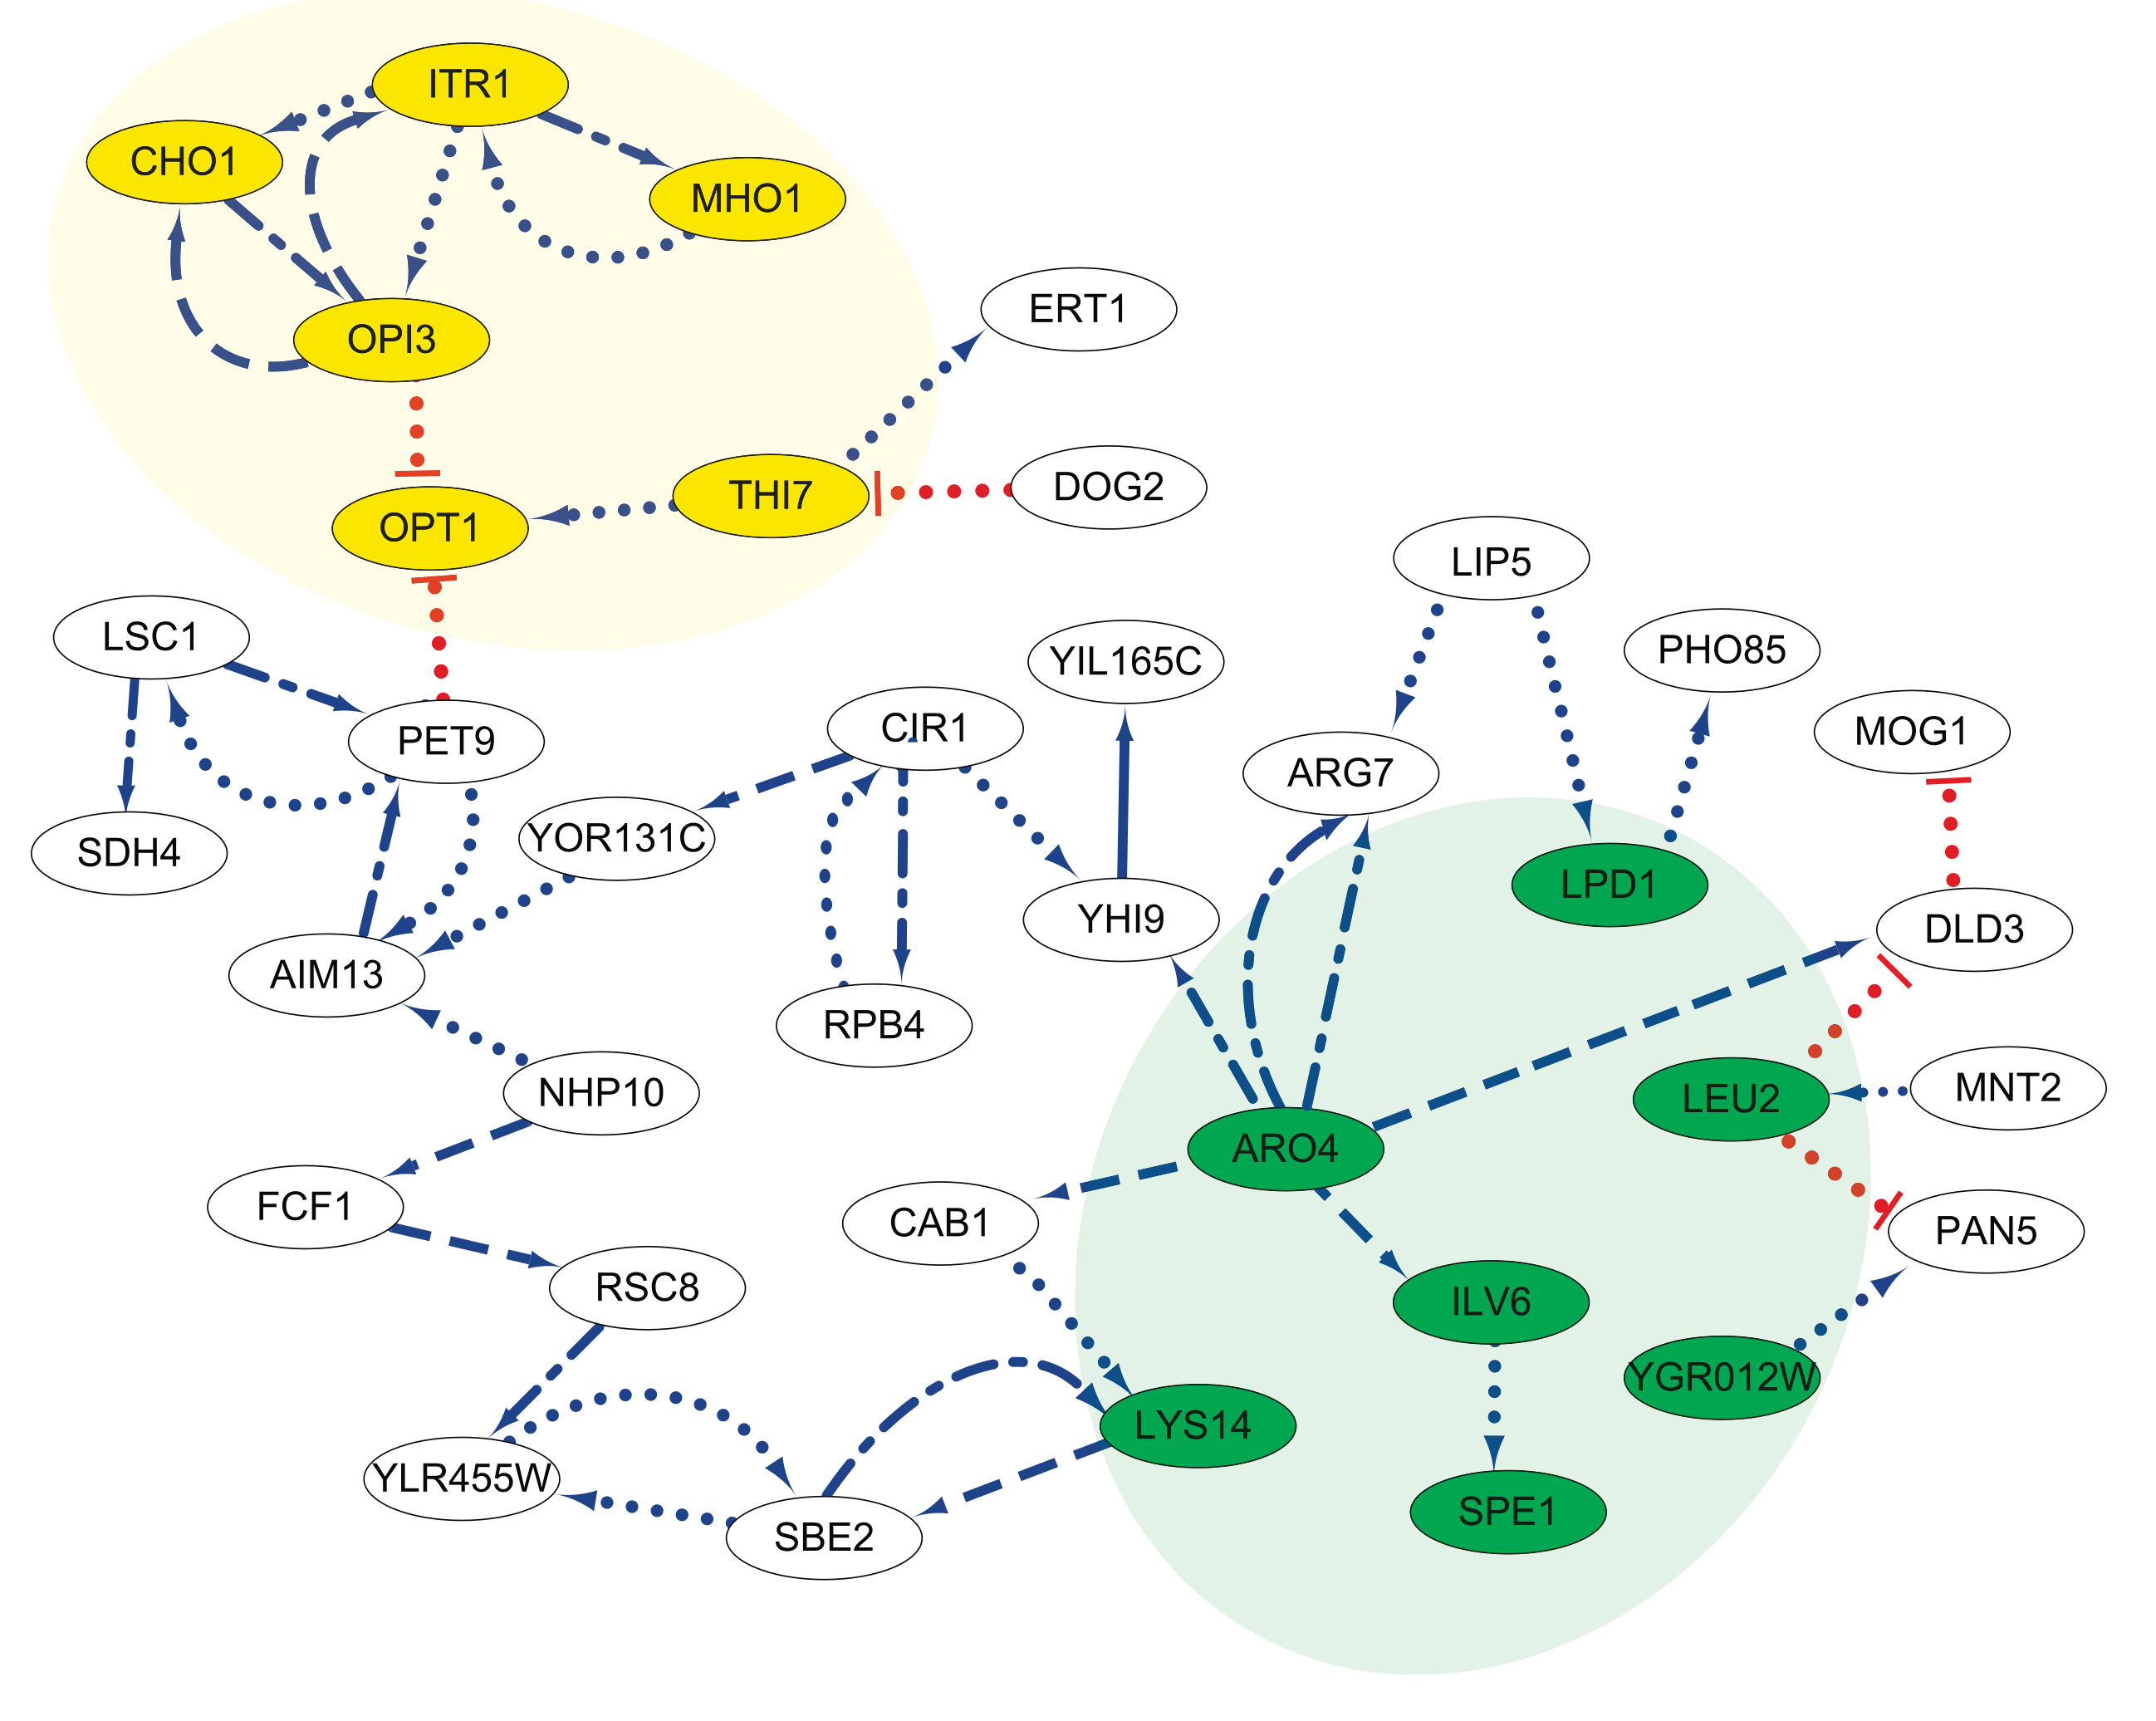
\includegraphics[width=.4\textwidth]{\fignet/CZH19-Nature-Fig1}
    \end{tabular}
  \end{tabular}

}

% %------------------------------------------------------------------------------
% \frame{ \frametitle{Two main situations}
% 
%   \paragraph{Network not observed:} 
%   we aim at reconstructing it
%   $$
%   \rightarrow \text{'network inference'}
%   $$
%   
%   \bigskip \bigskip \pause
%   \paragraph{Observed network:} 
%   we aim at understanding it
%   $$
%   \rightarrow \text{'network analysis'}
%   $$
% }
% 


%-------------------------------------------------------------------------------
%-------------------------------------------------------------------------------
\section{Network inference: a brief introduction}
%-------------------------------------------------------------------------------
%-------------------------------------------------------------------------------

%-------------------------------------------------------------------------------
\frame{ \frametitle{Typical aim}

  $$
  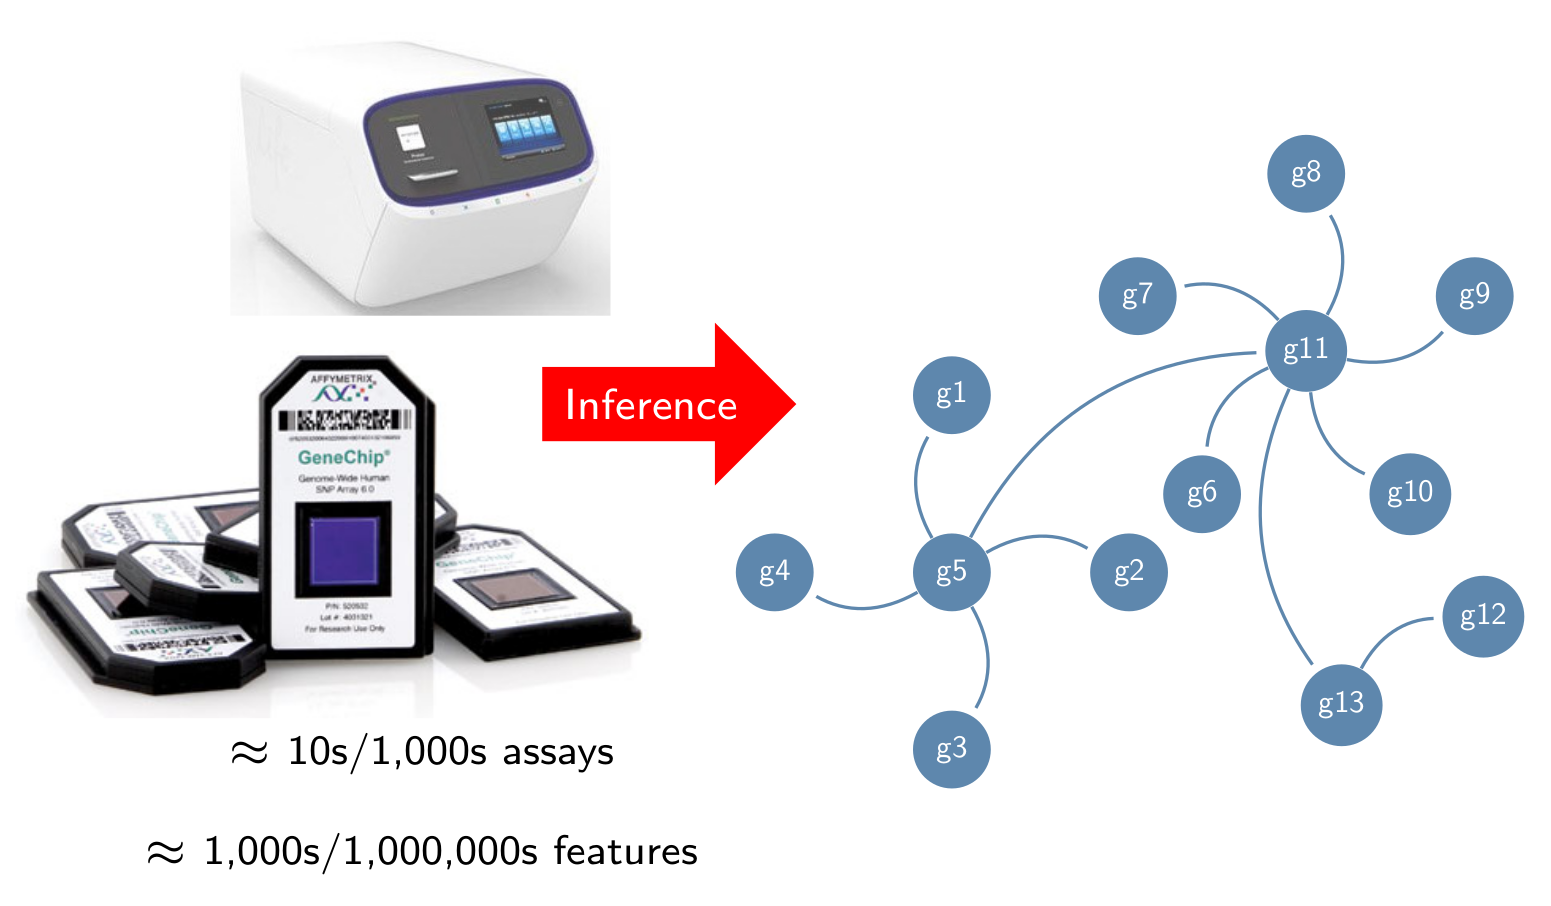
\includegraphics[width=.65\textwidth]{\fignet/Chi18-JC2BIM-p7}
  $$

  \pause
  That is, 
  \begin{itemize}
    \item go from gene expression $Y$ measurements to a gene network $G$ \\
      (replace 'gene' with 'microbe', 'neurone', ...), 
    \item i.e. go from information collected on the nodes to connexions between them.
  \end{itemize}

}

%-------------------------------------------------------------------------------
\frame{ \frametitle{Statistical model}

  \paragraph{Observed data.} The expression vector for sample $i$:
  $$
  y_i = [y_{i1} \dots y_{ij} \dots y_{ip}]
  $$
  is seen as a realisation of a random vector
  $$
  Y_i = [Y_{i1} \dots Y_{ij} \dots Y_{ip}]
  $$

  \bigskip \pause
  \paragraph{Statistical model.} 
  $$
  Y_i \sim p
  $$

  \bigskip \bigskip \pause
  \paragraph{Where is the network (graph)?} \\ ~
  \begin{itemize}
    \item The graph $G$ has to be encoded in the distribution $p$ in some way \\ ~
    \item \emphase{Graphical models} establish a formal connexion between $p$ and $G$
  \end{itemize}

  
}

%-------------------------------------------------------------------------------
%-------------------------------------------------------------------------------
\subsection{Graphical models}
%-------------------------------------------------------------------------------
\frame{\frametitle{Graphical models} 

  \bigskip
  \paragraph{'Interaction':} 
  need for a probabilistic / statistical counterpart for this concept

  \bigskip 
  \paragraph{Translation:} 
  $$
  \text{interactions} 
  := 
  \text{dependency structure of a set of random variables}
  $$

  \pause\bigskip
  \begin{tabular}{lll}
    \paragraph{Graphical models:} &
    \paragraph{Directed models.} ~ &
    \paragraph{Undirected models.} ~ \\
    \begin{tabular}{p{0.3\textwidth}} A generic \\ framework \\ \refer{Lau96,WaJ08}
    \end{tabular}
    & 
    \begin{tabular}{p{0.3\textwidth}}   \begin{tikzpicture}
    \node[observed] (a) at (.5*\edgeunit, 2.75*\edgeunit) {$A$};
  \node[observed] (b) at (0*\edgeunit, 2*\edgeunit) {$B$};
  \node[observed] (c) at (1*\edgeunit, 2*\edgeunit) {$C$};
  \node[observed] (d) at (0.5*\edgeunit, 1*\edgeunit) {$D$};
  \node[observed] (e) at (0*\edgeunit, 0*\edgeunit) {$E$};
  \node[observed] (f) at (1*\edgeunit, 0*\edgeunit) {$F$};

  
  \draw[arrow] (a) to (b);  \draw[arrow] (a) to (c);
  \draw[arrow] (b) to (d);  \draw[arrowbendleft] (b) to (f);
  \draw[arrow] (c) to (d);  \draw[arrow] (d) to (e);
  \draw[arrow] (d) to (f);  
  \end{tikzpicture}
 \end{tabular}
    & 
    \begin{tabular}{p{0.3\textwidth}}   \begin{tikzpicture}
  %   \node[observed] (a) at (0.75*\edgeunit, 1.5*\edgeunit) {$A$};
%   \node[observed] (b) at (0*\edgeunit, 0.75*\edgeunit) {$B$};
%   \node[observed] (c) at (0.75*\edgeunit, 0*\edgeunit) {$C$};
%   \node[observed] (d) at (1.5*\edgeunit, 0.75*\edgeunit) {$D$};
%   \node[observed] (e) at (2.25*\edgeunit, 0*\edgeunit) {$E$};
%   \node[observed] (f) at (3*\edgeunit, 0.75*\edgeunit) {$F$};
%   \node[observed] (g) at (2.25*\edgeunit, 1.5*\edgeunit) {$G$};

  \node[observed] (a) at (.5*\edgeunit, 3*\edgeunit) {$A$};
  \node[observed] (b) at (0*\edgeunit, 2.25*\edgeunit) {$B$};
  \node[observed] (c) at (1*\edgeunit, 2.25*\edgeunit) {$C$};
  \node[observed] (d) at (0.5*\edgeunit, 1.5*\edgeunit) {$D$};
  \node[observed] (e) at (0*\edgeunit, .75*\edgeunit) {$E$};
  \node[observed] (f) at (1*\edgeunit, .75*\edgeunit) {$F$};
  \node[observed] (g) at (.5*\edgeunit, 0*\edgeunit) {$G$};

  
  \draw[edge] (a) to (b);  \draw[edge] (a) to (c);  \draw[edge] (a) to (d);
  \draw[edge] (b) to (c);  \draw[edge] (b) to (d);  \draw[edge] (c) to (d);
  \draw[edge] (d) to (e);  \draw[edge] (d) to (f);  \draw[edge] (e) to (f);
  \draw[edge] (f) to (g);  
  \end{tikzpicture}

 \end{tabular}
    \end{tabular}
  }

%==================================================================
\frame{\frametitle{Undirected graphs = Markov random fields}

  \paragraph{Definition.} Let $G$ be an {\sl undirected graph}, the distribution $p$ is said faithful to $G$ if
  $$
  p(y_1, \dots y_n) \propto \prod_{C \in \Ccal(G)} \psi_C(y_C).
  $$
  where $\Ccal(G)$ is the set of (maximal) cliques of $G$

  \bigskip \bigskip \pause
  \begin{tabular}{cc}
    \begin{tabular}{c}
    $  \begin{tikzpicture}
  %   \node[observed] (a) at (0.75*\edgeunit, 1.5*\edgeunit) {$A$};
%   \node[observed] (b) at (0*\edgeunit, 0.75*\edgeunit) {$B$};
%   \node[observed] (c) at (0.75*\edgeunit, 0*\edgeunit) {$C$};
%   \node[observed] (d) at (1.5*\edgeunit, 0.75*\edgeunit) {$D$};
%   \node[observed] (e) at (2.25*\edgeunit, 0*\edgeunit) {$E$};
%   \node[observed] (f) at (3*\edgeunit, 0.75*\edgeunit) {$F$};
%   \node[observed] (g) at (2.25*\edgeunit, 1.5*\edgeunit) {$G$};

  \node[observed] (a) at (.5*\edgeunit, 3*\edgeunit) {$A$};
  \node[observed] (b) at (0*\edgeunit, 2.25*\edgeunit) {$B$};
  \node[observed] (c) at (1*\edgeunit, 2.25*\edgeunit) {$C$};
  \node[observed] (d) at (0.5*\edgeunit, 1.5*\edgeunit) {$D$};
  \node[observed] (e) at (0*\edgeunit, .75*\edgeunit) {$E$};
  \node[observed] (f) at (1*\edgeunit, .75*\edgeunit) {$F$};
  \node[observed] (g) at (.5*\edgeunit, 0*\edgeunit) {$G$};

  
  \draw[edge] (a) to (b);  \draw[edge] (a) to (c);  \draw[edge] (a) to (d);
  \draw[edge] (b) to (c);  \draw[edge] (b) to (d);  \draw[edge] (c) to (d);
  \draw[edge] (d) to (e);  \draw[edge] (d) to (f);  \draw[edge] (e) to (f);
  \draw[edge] (f) to (g);  
  \end{tikzpicture}

$
    \end{tabular}
    &
    \begin{tabular}{p{.7\textwidth}}
      \begin{eqnarray*}
%         p(a, \dots g) & \propto 
%         & \psi_1(a, b, c) \; \psi_2(a, b, d) \; \psi_3(a, c, d) \; \psi_4(b, c, d) \\
%         & & \psi_5(d, e, f) \; \psi_6(f, g) \\\pause
%       \text{but also} \qquad \\
        p(a, \dots g) & \propto 
        & \psi_1(a, b, c, d) \\
        & & \psi_2(d, e, f) \; \psi_3(f, g) 
      \end{eqnarray*}
%       \ra Only consider \emphase{maximal} cliques
    \end{tabular}
  \end{tabular}
}

%====================================================================
\frame{\frametitle{Conditional independence}

  \paragraph{Property.} If $p(y) > 0$, 
  $$
  \text{separation} \qquad \Leftrightarrow \qquad \text{conditional independence}
  $$

  \bigskip \pause
  \begin{tabular}{ccc}
    \hspace{.2\textwidth} 
    &
    \begin{tabular}{c}
    $  \begin{tikzpicture}
  %   \node[observed] (a) at (0.75*\edgeunit, 1.5*\edgeunit) {$A$};
%   \node[observed] (b) at (0*\edgeunit, 0.75*\edgeunit) {$B$};
%   \node[observed] (c) at (0.75*\edgeunit, 0*\edgeunit) {$C$};
%   \node[observed] (d) at (1.5*\edgeunit, 0.75*\edgeunit) {$D$};
%   \node[observed] (e) at (2.25*\edgeunit, 0*\edgeunit) {$E$};
%   \node[observed] (f) at (3*\edgeunit, 0.75*\edgeunit) {$F$};
%   \node[observed] (g) at (2.25*\edgeunit, 1.5*\edgeunit) {$G$};

  \node[observed] (a) at (.5*\edgeunit, 3*\edgeunit) {$A$};
  \node[observed] (b) at (0*\edgeunit, 2.25*\edgeunit) {$B$};
  \node[observed] (c) at (1*\edgeunit, 2.25*\edgeunit) {$C$};
  \node[observed] (d) at (0.5*\edgeunit, 1.5*\edgeunit) {$D$};
  \node[observed] (e) at (0*\edgeunit, .75*\edgeunit) {$E$};
  \node[observed] (f) at (1*\edgeunit, .75*\edgeunit) {$F$};
  \node[observed] (g) at (.5*\edgeunit, 0*\edgeunit) {$G$};

  
  \draw[edge] (a) to (b);  \draw[edge] (a) to (c);  \draw[edge] (a) to (d);
  \draw[edge] (b) to (c);  \draw[edge] (b) to (d);  \draw[edge] (c) to (d);
  \draw[edge] (d) to (e);  \draw[edge] (d) to (f);  \draw[edge] (e) to (f);
  \draw[edge] (f) to (g);  
  \end{tikzpicture}

$
    \end{tabular}
    &
    \begin{tabular}{p{.7\textwidth}}
    \begin{itemize}
     \item $A \not\independent B$ \\ ~
     \item $A \not\independent D \mid B$ \\ ~
     \item $A \not\independent D \mid \{B, C\}$ \\ ~
     \item $\{A, B, C\} \independent \{E, F, G\} \mid D$ \\ ~
     \item $\{B, C\} \independent \{E, F\} \mid D$ \\ ~
    \end{itemize}
    \end{tabular}
  \end{tabular}

  \bigskip
  \ra Inferring $G$ = Inferring conditional {\sl dependences} = 'direct interactions'
}
  
%==================================================================
\frame{\frametitle{Recovering $G$ from $Y$: Not an easy task}

  \paragraph{A huge search space:}
  $$
  \includegraphics[trim=50 50 0 75, height=.5\textheight, clip]{\fignet/NbGraphs2}
  $$
  Number of \textcolor{darkgreen}{undirected graphs} ($2^{p(p-1)/2}$), \textcolor{red}{directed acyclic graphs} (no close form), \textcolor{blue}{spanning trees} ($p^{p-2}$)
  
  \bigskip \pause
  \paragraph{A common assumption:} 
  \begin{align*}
  \text{$G$ is sparse} \qquad 
  & \Leftrightarrow \qquad \text{Each node has few neighbors}   \\
  & \Leftrightarrow \qquad \text{Each gene directly interacts with few other genes} 
  \end{align*}
}

%==================================================================
\subsection*{Gaussian graphical models (GGM)}
%==================================================================

%==================================================================
\frame{\frametitle{Gaussian graphical models (GGM)}

  \paragraph{Gaussian setting.} Suppose that each 'expression' vector $Y_i = (Y_{i1} \dots Y_{ip})$ is Gaussian
  $$
  Y_i \sim \Ncal_p(\mu, \Sigma)
  $$
  \begin{itemize}
   \item $\mu = (p \times 1)$ vector of mean expressions
   \item $\Sigma = (p \times p)$ covariance matrix:
   $$
   \sigma_{jj} = \sigma_j^2 = \Var(Y_{ij}), \qquad
   \sigma_{jk} = \Cov(Y_{ij}, Y_{ik}), \qquad
   \rho_{jk} = \frac{\sigma_{jk}}{\sigma_j \sigma_k}
   $$
  \end{itemize}

  \bigskip \pause
  \paragraph{Property.}
  $$
  \text{null correlation} \quad \Leftrightarrow \qquad
  \text{null covariance} \quad \Leftrightarrow \qquad
  \text{independence} 
  $$
  i.e.
  $$
  \sigma_{jk} = 0 \quad \Leftrightarrow \qquad Y_{ij} \independent Y_{ik} 
  \pause \emphase{\text{ marginally}}
  $$
}

%==================================================================
\frame{\frametitle{Regression point of view}

  \paragraph{Gene-by-gene approach:} Finding the neighbors of a node is equivalent to find its 'parents' in a regression:
  $$
  Y_{ik} = \sum_{j \neq k} \beta_{jk} Y_{ij} + E_{ik}.
  $$
  \ra Requires a testing procedure \refer{VeV09} or a penalization \refer{MeB06} to determine non-zero coefficients

  \bigskip \bigskip \pause
  \paragraph{Remarks.}
  \begin{itemize}
   \item Regression needs reconciliation when $\widehat{\beta}_{jk} = 0$ and $\widehat{\beta}_{jk} \neq 0$ 
   \item \refer{Ver12} provides bounds for the recovery of the list of neighbors: let $d =$ degree of a given node 
   \begin{align*}
    d \log(p/d) & \leq n & & \text{possible recovery} \\
    d \log(p/d) & > n \log n & & \text{impossible recovery}
   \end{align*}
  \end{itemize}
}

%==================================================================
\frame{\frametitle{A nice property of GGM's}

  \begin{tabular}{cc}
    \begin{tabular}{p{.5\textwidth}}
    \hspace{-.15\textwidth}
    \includegraphics[width=.6\textwidth]{\fignet/FigGGM-4nodes}
    \end{tabular}
    & 
    \hspace{-.15\textwidth}
    \begin{overprint}
    \onslide<2>
    \begin{tabular}{p{.5\textwidth}}
	 \paragraph{Graphical model.}
	 $$
	 G = \left[ \begin{array}{cccc}
	 0 & 1 & 1 & \emphase{0} \\
	 1 & 0 & 1 & \emphase{0} \\
	 1 & 1 & 0 & 1 \\
	 \emphase{0} & \emphase{0} & 1 & 0 
	 \end{array} \right]
	 $$
	 \bigskip
	 \begin{itemize}
	  \item Connected \\ ~
	  \item 3 separates 4 from (1, 2)
	 \end{itemize}
    \end{tabular} 
    \onslide<3>
    \begin{tabular}{p{.5\textwidth}}
	 \paragraph{Covariance matrix.}
	 $$
	 \Sigma \propto \left[ \begin{array}{cccc}
	   1 & -.25 & -.41 &  \emphase{.25} \\
	   -.25 &  1 & -.41 &  \emphase{.25} \\
	   -.41 & -.41 &  1 & -.61 \\
	   \emphase{.25} &  \emphase{.25} & -.61 &  1
	   \end{array} \right] 
	 $$
	 \bigskip
	 \begin{itemize}
	  \item No zero because $G$ is Connected
	 \end{itemize}
    \end{tabular} 
    \onslide<4>
    \begin{tabular}{p{.5\textwidth}}
	 \paragraph{Inverse covariance matrix.}
	 $$
	 \Sigma^{-1} \propto \left[ \begin{array}{cccc}
	   1 & .5 & .5 & \emphase{0} \\
	   .5 & 1 & .5 & \emphase{0} \\
	   .5 & .5 & 1 & .5 \\
	   \emphase{0} & \emphase{0} & .5 & 1
	   \end{array} \right] 
	 $$
	 \bigskip
	 \begin{itemize}
	  \item 0's at (1, 4) and (2, 4)\\ ~
	  \item Conditional independence\\ ~
	  \item $\Omega := \Sigma^{-1} =$ \emphase{precision} matrix
	 \end{itemize}
    \end{tabular} 
    \end{overprint}
  \end{tabular}

}

%==================================================================
\frame{\frametitle{More formally}

  \paragraph{If $Y \sim \Ncal(0, \Omega^{-1})$,} then
  \begin{align*}
  p(Y) & \propto \exp\left(-\frac12 \|Y\|^2_\Omega \right)\\
  & = \exp\left(-\frac12 \sum_{j, k} \omega_{jk} Y_j Y_k\right)  
  & & \text{where } \Omega = [\omega_{jk}] \\
  & = \prod_{j, k} \underset{\phi_{jk}(Y_j, Y_k)}{\underbrace{\exp\left(-\frac12 \omega_{jk} Y_j Y_k\right)}}
  \end{align*}

  \bigskip \pause
  \begin{itemize}
   \item The non-zeros of $\Omega$ correspond to the edges of $G$\\ ~
   \item Furthermore:
   $$
   - \omega_{jk} \; \propto \; 
   \Cor\left(Y_j, Y_k \mid Y_{\{j, k\}}\right)
   = \text{ \emphase{'partial'} correlation}
   $$
  \end{itemize}
  
}

%==================================================================
\frame{\frametitle{Inference}

\begin{tabular}{cc}
    \begin{tabular}{p{.5\textwidth}}
    \hspace{-.15\textwidth}
    \includegraphics[width=.6\textwidth]{\fignet/FigGGM-4nodes}
    \end{tabular}
    & 
    \hspace{-.15\textwidth}
    \begin{overprint}
    \onslide<1>
    \begin{tabular}{p{.5\textwidth}}
	 \paragraph{Graphical model.}
	 $$
	 G = \left[ \begin{array}{cccc}
	 0 & 1 & 1 & \emphase{0} \\
	 1 & 0 & 1 & \emphase{0} \\
	 1 & 1 & 0 & 1 \\
	 \emphase{0} & \emphase{0} & 1 & 0 
	 \end{array} \right]
	 $$
    \end{tabular} 
    \onslide<2>
    \begin{tabular}{p{.5\textwidth}}
	 \paragraph{Inverse covariance matrix.}
	 $$
	 \Omega \propto \left[ \begin{array}{cccc}
	   1 & .5 & .5 & \emphase{0} \\
	   .5 & 1 & .5 & \emphase{0} \\
	   .5 & .5 & 1 & .5 \\
	   \emphase{0} & \emphase{0} & .5 & 1
	   \end{array} \right] 
	 $$
	 \bigskip
	 \begin{itemize}
	  \item Same zeros as $G$
	 \end{itemize}
    \end{tabular} 
    \onslide<3>
    \begin{tabular}{p{.5\textwidth}}
	 \paragraph{Estimated inverse covariance matrix.}
	 $$
	 \widehat{\Omega} \propto \left[ \begin{array}{cccc}
	   1 & .48 & .61 & \emphase{.09} \\
	   .48 & 1 & .67 & \emphase{.06} \\
	   .61 & .67 & 1 & .46 \\
	   \emphase{.09} & \emphase{.06} & .46 & 1
	   \end{array} \right] 
	 $$
	 ($n = 100$)
	 \bigskip
	 \begin{itemize}
	  \item No 'true zero' in the estimate\\ ~
	  \item Need to 'force' zeros to appear
	 \end{itemize}
    \end{tabular} 
    \end{overprint}
  \end{tabular}
}

%==================================================================
\frame{\frametitle{Making $\Omega$ sparse}

  \paragraph{Graphical lasso \refer{FHT08}.} Penalized likelihood:
  $$
  \max_{\mu, \Omega} \log p(Y; \mu, \Omega) - \lambda \sum_{j < k} |\omega_{jk}|
  $$
  the '$\ell_1$' penalty ($|\omega_{jk}|$) forces some $\omega_{jk}$ to be zero. \\
  \ra The higher $\lambda$, the sparser $\widehat{G}$ \\
  \ra Again a convex problem \\
  \ra Fast solution (e.g. {\tt huge} R package)
  
  \bigskip \bigskip \pause
  \paragraph{Playing with penalties.}
  \begin{itemize}
   \item Other forms of penalties ($\ell_1$, $\ell_2$, combinations) induces other topologies
   \item Ex.: \refer{ACM09} induce clustered networks.
  \end{itemize}
  
  \bigskip \bigskip \pause
  \paragraph{Alternatives.}
  \begin{itemize}
   \item Mixture of tree-shaped distributions: \refer{MeJ06,Kir07,JFS16,ScR17,MRA19}
   \item ...
  \end{itemize}
}



%-------------------------------------------------------------------------------
%-------------------------------------------------------------------------------
\section{Network inference from count data}
%-------------------------------------------------------------------------------
%-------------------------------------------------------------------------------

%------------------------------------------------------------------------------
\frame{ \frametitle{Dealing with count data}

  \paragraph{Sequencing technology} provide count data, that is numbers of reads mapping to
  \begin{itemize}
    \item a gene (expression)
    \item an OTU (metagenomics)
    \item \dots
  \end{itemize}

  \bigskip \bigskip \pause
  \paragraph{Non-Gaussian data.} 
  \begin{itemize}
    \item The normal distribution does not fit count (or presence/absence) data \\ ~
    \item Not many flexible {\sl multivariate} distributions for count or binary data do exist \refer{IYA17}
  \end{itemize}

  \bigskip \bigskip \pause
  \paragraph{A common trick:} latent variable models
  \begin{itemize}
%     \item See \refer{WBO15} for an introduction for species abundance distributions 
    \item Most popular structure = latent GGM: 
    Spiec-Easi \refer{KMM15}, gCODA \refer{FHZ17}, MiNT \refer{BML16}, PLNnetwork \refer{CMR18b} %, tree-based PLN \refer{MRA19}  
    \\ ~
    \item Next: focus on PLNnetwork (abundance data)
  \end{itemize}

}


%==================================================================
\frame{\frametitle{Poisson log-normal model}

  \paragraph{Data:} $n$ independent samples (no spatial structure), $p$ 'genes', 
  $$
  Y_{ij} = \text{ count for gene $j$ in sample $i$}
  $$
  
  \bigskip \pause
  \paragraph{Poisson log-normal (PLN) model \refer{AiH89}:} 
  \begin{itemize}
   \item For each sample, draw independently
   $$
   Z_i \sim \Ncal_p(0, \Omega^{-1})
   $$
   \item \pause For each gene in each sample, draw independently (given $Z$)
   $$
   Y_{ij} \mid Z_{ij} \sim \Pcal(\exp(\mu_j + Z_{ij}))
   $$
  \end{itemize} \pause
  summarized as
  $$
  \{Y_i\} \text{ iid} \sim PLN(\mu, \Omega^{-1})
  $$

  \bigskip \pause
  \paragraph{Interpretation.}
  \begin{itemize}
%   \item PLN is a mixed model
  \item $\mu_j =$ mean (log-)count of gene $j$
  \item $\Omega = $ dependency structure (encoded in the latent layer)
  \end{itemize}
}

%==================================================================
\frame{\frametitle{Multivariate Poisson log-normal distribution}

  \paragraph{Some (desirable) properties.} \refer{AiH89} \\~
  \begin{itemize}
    \item Prediction:
    $$
    \Esp(Y_{ij}) = \exp(\mu_j + \sigma^2_j/2)
    $$ 
    where $\sigma^2_j = \Var(Z_{ij})$ \\~
    \item Overdispersion:
    \begin{align*}
    \Var(Y_{ij}) 
    = \Esp(Y_{ij}) + \Esp^2(Y_{ij}) (e^{\sigma^2_j} - 1)
    %  > \Var(\Pcal(\exp(x_i^\intercal \beta_j + \sigma^2_j/2)) 
    \qquad > \qquad \Var(\text{Poisson})
    \end{align*} \\~
    \item Correlations sign:
    $$
    \sign(\Cor(Z_{ij}, Z_{ik})) = \sign(\Cor(Y_{ij}, Y_{ik})) 
    $$
  \end{itemize}

  

}

%==================================================================
\frame{\frametitle{PLNnetworks}

  \paragraph{PLN network model.} Same model as PLN + sparsity assumption:
  $$
  \{Y_i\} \text{ iid} \sim PLN(\mu, \Omega)
  \qquad \qquad + \emphase{\Omega \text{ sparse}}
  $$
  
  \bigskip \bigskip \pause
  \paragraph{Inference algorithm.} Variational EM + sparsity inducing norm \refer{CMR18b,CMR19}:
  $$
  \max_{\mu, \Omega} \widetilde{\log p}(Y; \mu, \Omega) - \lambda \sum_{j < k} |\omega_{jk}|
  $$
  \ra Alternate convex problems \\
  \ra Fast solution ({\tt PLNmodels} R package)
  
  \bigskip
  \begin{itemize}
   \item Resampling (StARS \refer{LRW10}) is highly recommended to assess edge robustness
  \end{itemize}
}

%==================================================================
\frame{\frametitle{Latent network}

  \paragraph{Some undesirable property:} {all latent (GGM) models} infer the dependency struture of the latent $Z$, not of the observed abundances $Y$
  
  \bigskip \bigskip 
  \renewcommand{\nodesize}{2em}
  \begin{overprint}
    \onslide<2>
    $$
    \begin{array}{ccc}
    p(Z, Y) & & p(Y) \\ ~\\
      \begin{tikzpicture}[scale=.8]
  \node[hidden] (Z1) at ( 0.95*\edgeunit,  0.31*\edgeunit) {$Z_1$};
  \node[hidden] (Z2) at (-0.00*\edgeunit,  1.00*\edgeunit) {$Z_2$};
  \node[hidden] (Z3) at (-0.95*\edgeunit,  0.31*\edgeunit) {$Z_3$};
  \node[hidden] (Z4) at (-0.59*\edgeunit, -0.81*\edgeunit) {$Z_4$};
  \node[hidden] (Z5) at ( 0.59*\edgeunit, -0.81*\edgeunit) {$Z_5$};
  
  \draw[edge] (Z1) to (Z5);  \draw[edge] (Z2) to (Z3);  
  \draw[edge] (Z2) to (Z4);  \draw[edge] (Z3) to (Z4); 

  \node[observed] (Y1) at ( 1.05*\edgeunit, -0.39*\edgeunit) {$Y_1$};
  \node[observed] (Y2) at (-0.00*\edgeunit,  0.30*\edgeunit) {$Y_2$};
  \node[observed] (Y3) at (-1.05*\edgeunit, -0.39*\edgeunit) {$Y_3$};
  \node[observed] (Y4) at (-0.59*\edgeunit, -1.51*\edgeunit) {$Y_4$};
  \node[observed] (Y5) at ( 0.59*\edgeunit, -1.51*\edgeunit) {$Y_5$};
  
  \draw[arrow] (Z1) to (Y1); 
  \draw[arrow] (Z2) to (Y2);
  \draw[arrow] (Z3) to (Y3);
  \draw[arrow] (Z4) to (Y4);
  \draw[arrow] (Z5) to (Y5);
  \end{tikzpicture}

    & \qquad \qquad &
      \begin{tikzpicture}[scale=.8]
  \node[observed] (Y1) at ( 0.95*\edgeunit,  0.31*\edgeunit) {$Y_1$};
  \node[observed] (Y2) at (-0.00*\edgeunit,  1.00*\edgeunit) {$Y_2$};
  \node[observed] (Y3) at (-0.95*\edgeunit,  0.31*\edgeunit) {$Y_3$};
  \node[observed] (Y4) at (-0.59*\edgeunit, -0.81*\edgeunit) {$Y_4$};
  \node[observed] (Y5) at ( 0.59*\edgeunit, -0.81*\edgeunit) {$Y_5$};
  \node[empty] (YY) at ( 0.59*\edgeunit, -1.51*\edgeunit) {};

  \draw[edge] (Y1) to (Y5);  \draw[edge] (Y2) to (Y3);  
  \draw[edge] (Y2) to (Y4);  \draw[edge] (Y3) to (Y4);  
  
  \end{tikzpicture}

    \end{array}
    $$
    \onslide<3>
    $$
    \begin{array}{ccc}
    p(Z, Y) & & p(Y) \\ ~\\
      \begin{tikzpicture}[scale=.8]
    \node[hidden] (Z1) at ( 0.95*\edgeunit,  0.31*\edgeunit) {$Z_1$};
    \node[hidden] (Z2) at (-0.00*\edgeunit,  1.00*\edgeunit) {$Z_2$};
    \node[hidden] (Z3) at (-0.95*\edgeunit,  0.31*\edgeunit) {$Z_3$};
    \node[hidden] (Z4) at (-0.59*\edgeunit, -0.81*\edgeunit) {$Z_4$};
    \node[hidden] (Z5) at ( 0.59*\edgeunit, -0.81*\edgeunit) {$Z_5$};
    
    \draw[edge] (Z1) to (Z2);  \draw[edge] (Z1) to (Z4);  
    \draw[edge] (Z1) to (Z5);  \draw[edge] (Z2) to (Z3);  
    \draw[edge] (Z2) to (Z4);  \draw[edge] (Z3) to (Z4); 

    \node[observed] (Y1) at ( 1.05*\edgeunit, -0.39*\edgeunit) {$Y_1$};
    \node[observed] (Y2) at (-0.00*\edgeunit,  0.30*\edgeunit) {$Y_2$};
    \node[observed] (Y3) at (-1.05*\edgeunit, -0.39*\edgeunit) {$Y_3$};
    \node[observed] (Y4) at (-0.59*\edgeunit, -1.51*\edgeunit) {$Y_4$};
    \node[observed] (Y5) at ( 0.59*\edgeunit, -1.51*\edgeunit) {$Y_5$};

    \draw[arrow] (Z1) to (Y1); 
    \draw[arrow] (Z2) to (Y2);
    \draw[arrow] (Z3) to (Y3);
    \draw[arrow] (Z4) to (Y4);
    \draw[arrow] (Z5) to (Y5);
  \end{tikzpicture}

    & \qquad \qquad &
      \begin{tikzpicture}[scale=.8]
  \node[observed] (Y1) at ( 0.95*\edgeunit,  0.31*\edgeunit) {$Y_1$};
  \node[observed] (Y2) at (-0.00*\edgeunit,  1.00*\edgeunit) {$Y_2$};
  \node[observed] (Y3) at (-0.95*\edgeunit,  0.31*\edgeunit) {$Y_3$};
  \node[observed] (Y4) at (-0.59*\edgeunit, -0.81*\edgeunit) {$Y_4$};
  \node[observed] (Y5) at ( 0.59*\edgeunit, -0.81*\edgeunit) {$Y_5$};
  \node[empty] (YY) at ( 0.59*\edgeunit, -1.51*\edgeunit) {};

  \draw[edge] (Y1) to (Y2);  \draw[edge] (Y1) to (Y3);  
  \draw[edge] (Y1) to (Y4);  \draw[edge] (Y1) to (Y5);  
  \draw[edge] (Y2) to (Y3);  \draw[edge] (Y2) to (Y4); 
  \draw[edge] (Y2) to (Y5);  \draw[edge] (Y3) to (Y4);  
  \draw[edge] (Y3) to (Y5);  \draw[edge] (Y4) to (Y5);  
  \end{tikzpicture}

    \end{array}
    $$
  \end{overprint}
  \renewcommand{\nodesize}{\commonnodesize}
}

%==================================================================
\frame{\frametitle{Sampling effort and covariates}

  \paragraph{Accounting for the sampling effort.} Read counts depend on the sampling effort.
  
  \bigskip \pause
  \ra Standard way to account for varying effort across samples: offset
  $$
  Y_{ij} \mid Z_{ij} \sim \Pcal(\exp(o_{ij} + \mu_j + Z_{ij}))
  $$
  where, e.g.
  $$
  o_{ij} = \log(\text{total read count in sample $i$})
  $$

  \bigskip \bigskip \pause
  \paragraph{Accounting for experimental conditions.} Gene expressions depend on experimental conditions.
  
  \bigskip \pause
  \ra Standard way to account for 'covariates' across samples: regression
  $$
  Y_{ij} \mid Z_{ij} \sim \Pcal(\exp(\textcolor{gray}{o_{ij} +\xspace} x_i^\intercal \beta_j + \mu_j + Z_{ij}))
  $$
  where, 
  \begin{align*}
    x_i & = [x_{i1} \dots x_{id}] & & \text{covariates for sample $i$} \\
    \beta_j & = [\beta_{j1} \dots \beta_{jd}] & & \text{regression coefficients for gene $j$}
  \end{align*}

}


%==================================================================
\frame{\frametitle{Barents fishes}

  \paragraph{Species abundance data:} 
  \begin{itemize}
    \item $n = 89$ sites (stations) in the Barents see (same sampling effort: no offset), \\ ~
    \item $p = 30$ fish species, \\ ~
    \item $d = 4$ covariates (latitude, longitude, depth, temperature) 
  \end{itemize}
  
  \bigskip \bigskip \pause
  \paragraph{Aims:} 
  \begin{itemize}
    \item Determine which pairs of species are in 'direct interaction' \\ ~
    \item Avoid 'spurious' edge due to environmental variations \\~ 
%     \item + Understand the effect of the sparsity penalty $\lambda$.
  \end{itemize}

}
  
%==================================================================
\frame{\frametitle{Barents fishes}

  \begin{center}
  \begin{tabular}{lccc}
    & no covariate & \textcolor{blue}{temp. \& depth} & \textcolor{red}{all covariates} \\
    \hline
    \rotatebox{90}{$\qquad\quad\lambda=.20$} &
    \includegraphics[width=.22\textwidth]{\figCMR/network_BarentsFish_Gnull_full60edges} &
    \includegraphics[width=.22\textwidth]{\figCMR/network_BarentsFish_Gsel_full60edges} &
    \includegraphics[width=.22\textwidth]{\figCMR/network_BarentsFish_Gfull_full60edges} 
    \vspace{-0.05\textheight} \pause \\ \hline
    %
    \rotatebox{90}{$\qquad\quad\lambda=.28$} &
    \includegraphics[width=.22\textwidth]{\figCMR/network_BarentsFish_Gnull_sel60edges} & \includegraphics[width=.22\textwidth]{\figCMR/network_BarentsFish_Gsel_sel60edges} &
    \includegraphics[width=.22\textwidth]{\figCMR/network_BarentsFish_Gfull_sel60edges} 
    \vspace{-0.05\textheight} \pause \\ \hline
    %
    \rotatebox{90}{$\qquad\quad\lambda=.84$} &
    \includegraphics[width=.22\textwidth]{\figCMR/network_BarentsFish_Gnull_null60edges} &
    \includegraphics[width=.22\textwidth]{\figCMR/network_BarentsFish_Gsel_null60edges} &
    \includegraphics[width=.22\textwidth]{\figCMR/network_BarentsFish_density} 
%     \includegraphics[width=.22\textwidth]{\figCMR/network_BarentsFish_Gfull_null60edges}  
  \end{tabular}
  \end{center}

}

%==================================================================
\frame{\frametitle{Oak mildew (1/2)}

  \paragraph{Metagenomic data:} 
  \begin{itemize}
    \item $n = 78$ samples collected on leaves from two trees (one susceptible to oak mildew, one resistant), \\ ~
    \item $p = 114$ OTUs: 66 bacteria + 48 fungi (inc. the pathogen {\sl E. alphitoides}  'f19'), \\ ~
    \item separate sequencing for bacteria and fungi: offset specific to each sample $i$ and OTU type
  \end{itemize}
  
  \bigskip \bigskip \pause
  \paragraph{Inferred networks:} 
  $$
  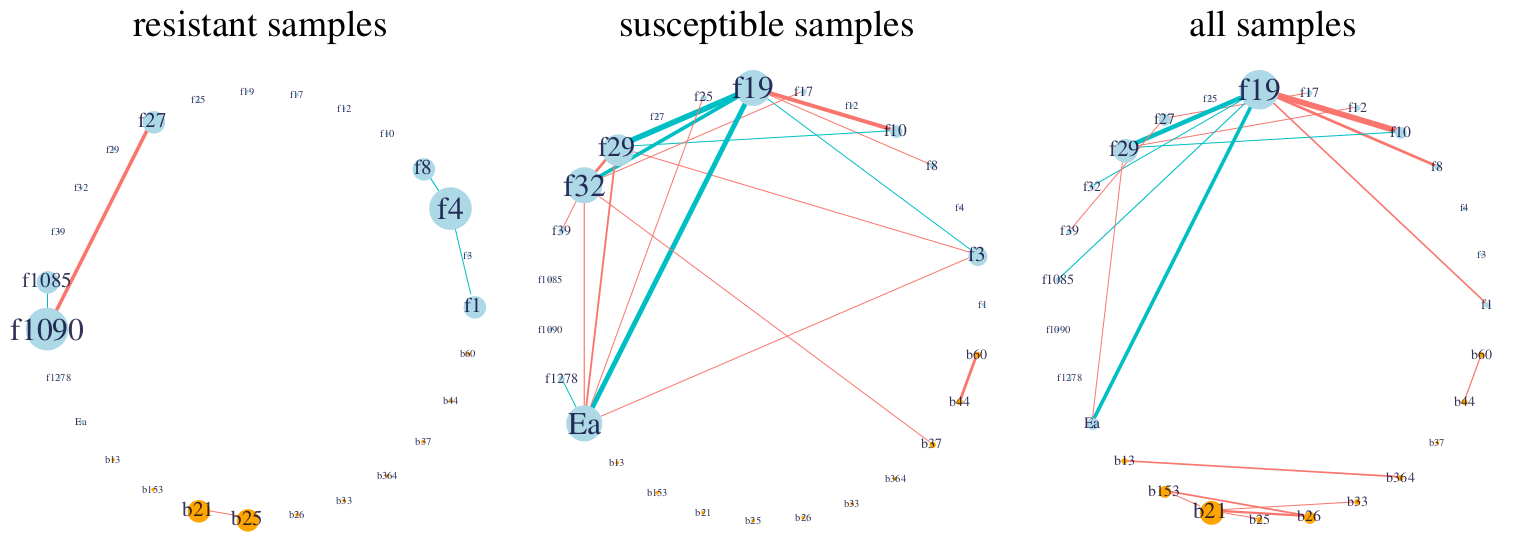
\includegraphics[width=.8\textwidth]{\fignet/CMR19-ICML-Fig3a}
  $$

}

%==================================================================
\frame{\frametitle{Oak mildew (2/2)}

  \begin{tabular}{cc}
    \hspace{-.04\textwidth}
    \begin{tabular}{p{.45\textwidth}}   
      \paragraph{Model selection.} As $\lambda$ decreases:
      \begin{itemize}
       \item the log-likelihood increases
       \item the number of parameters increases
      \end{itemize}
      
      \bigskip \bigskip 
      \paragraph{Penalized likelihood} criterion
      \begin{itemize}
       \item BIC
       \item EBIC
      \end{itemize}      
            
      \bigskip \bigskip 
      \paragraph{Robustness assessment} via resampling.

    \end{tabular}
    &
    \hspace{-.05\textwidth}
    \begin{tabular}{p{.45\textwidth}}   
      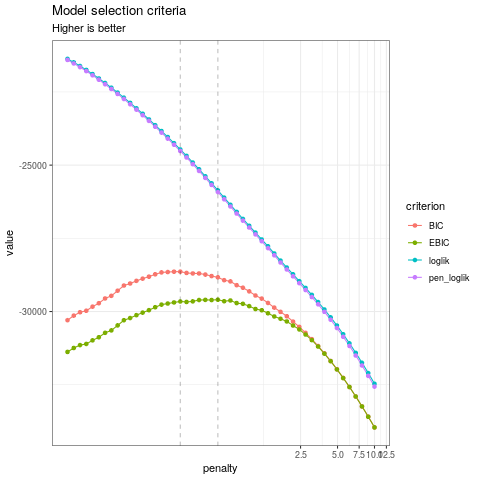
\includegraphics[width=.5\textwidth]{\fignet/JC2BIM-OaksPLN-netSel-full}
    \end{tabular}
  \end{tabular}


}


%-------------------------------------------------------------------------------
%-------------------------------------------------------------------------------
\section{Network analysis: looking for a structure}
%-------------------------------------------------------------------------------
%-------------------------------------------------------------------------------

%------------------------------------------------------------------------------
\frame{ \frametitle{Observed network}

  \begin{tabular}{ccc}
    \hspace{-.04\textwidth}
    \begin{tabular}{p{.35\textwidth}}
      \paragraph{Network} \\
      \includegraphics[width=.3\textwidth]{\fignet/SBM-Network}
    \end{tabular}
    & 
    \hspace{-.1\textwidth}
    \begin{tabular}{p{.35\textwidth}}
      \paragraph{Adjacency matrix} \\
      \includegraphics[width=.3\textwidth]{\fignet/SBM-Adjacency}
    \end{tabular}
    &
    \hspace{-.1\textwidth}
    \begin{tabular}{p{.35\textwidth}}
      \paragraph{That is}
      \begin{itemize}
        \item $n$ nodes (genes, proteins, species, \dots : $1 \leq i, j \leq n$) \\~
        \item $Y_{ij} = $ interaction between nodes $i$ and $j$
      \end{itemize}
    \end{tabular}
  \end{tabular}
  
  \bigskip \pause  
  $$
  \begin{tabular}{p{.35\textwidth}p{.35\textwidth}}
    \paragraph{Type of network:} & \paragraph{Type of edge:} \pause \\ %~ \\ 
    directed / undirected & $Y_{ij} = Y_{ji}$ or not \pause \\ %~ \\
    binary / valued ('weighted') & $Y_{ij} \in \{0, 1\}$ or $\Rbb$ \pause \\ %~ \\
    multivariate ('multiplex') & $Y_{ij} \in \{0, 1\}^d$ or $\Rbb^d$ \\ 
    & or $\{0, 1\} \times \{a, b, c, d\} \times \Nbb \times \Rbb$
  \end{tabular}     
  $$

}

%------------------------------------------------------------------------------
\frame{ \frametitle{Statistical model}

  \paragraph{Observed data.} The observed adjacency matrix 
  $$
  y = [y_{ij}]_{1 \leq i, j, \leq n}
  $$
  is a realisation of a {\sl random graph} (or random matrix)
  $$
  Y = [Y_{ij}]_{1 \leq i, j, \leq n}
  $$
  
  \bigskip \bigskip \pause
  \paragraph{Random graph model=} joint distribution of the $\approx n^2$ random values $Y_{ij}$ : 
  $$
  Y \sim p
  $$
  that is
  $$
  p(y) = \Pr\{Y_{11} = y_{11}, \dots Y_{ij} = y_{ij}, \dots Y_{nn} = y_{nn}\}
  $$

}

%==================================================================
\frame{ \frametitle{A simple random graph}

  \paragraph{Erd\"os-R\'enyi:}
  %\footnote{Alternate version $\Gcal(n, m)$, $m =$ fixed number of edges}:
  \begin{itemize}
   \item $n$ nodes (= genes, \dots) 
   \item undirected binary edges (= interactions) : $Y_{ij} = Y_{ji}  \in \{0, 1\}$
   \item all pairs of nodes are connected (= interact) independently 
   \item with same probability $\pi$
  \end{itemize}
  $$
  \{Y_{ij}\} \text{ iid } \sim \Bcal(\pi)
  $$
  
  \bigskip \bigskip \pause
  \paragraph{Properties.}
  \begin{itemize}
   \item Graph density $= \pi$ \\ ~
   \item Degree (= number of neighbors) of a node $\sim \Bcal(n-1, \pi) \approx \Pcal(n \pi)$ \\ ~
%    \ra Homegeneous degree distribution
   \item Clustering coefficient $c = P\{j \sim k \mid i \sim j, i \sim k\} = \pi$ %\\
   \qquad (no 'assortativity')
  \end{itemize}
}

%==================================================================
\frame{ \frametitle{Network analysis}

  \paragraph{Erd\"os-R\'enyi random graph.}
  \begin{itemize}
   \item Very well known and understood
   \item Does not fit most networks: all genes play exactly the same role
  \end{itemize}
  \ra Need for more complex models

  \bigskip \bigskip \pause
  \paragraph{Always the same:} What are we looking for ?
  
  \bigskip \pause
  \paragraph{Network topology (organization).}
  \begin{itemize}
  \item Node scale (degree distribution)
  \item Global scale (density, connected classes, \dots)
  \item Intermediate (e.g. node clustering: see next)
  \end{itemize}

  \bigskip \pause
  \paragraph{Network 'behavior':} e.g. is the network stable
  \begin{itemize}
  \item Relies on an implicit dynamic model
  \end{itemize}
  \ra Do we have the data to fit it?
}

%==================================================================
\frame{ \frametitle{Stochastic blockmodel}

  \bigskip
  \paragraph{Mixture model \refer{HoL79,NoS01}.} Undirected, binary version : 
  \begin{itemize}
    \item There exists $K$ groups of nodes \\~
    \item Each node $i$ belongs to one {\sl unobserved} class $Z_i$ \\~ 
    \item The probability for nodes $i$ and $j$ to be connected only depends on their respective groups :
    $$
    \Pr\{Y_{ij} \mid i \in k, j \in \ell\} = \gamma_{k\ell}
    $$
  \end{itemize}
  
  \bigskip \bigskip \pause
  \paragraph{Many avatars.} 
  \begin{itemize}
    \item Bipartite networks \refer{GoN05}, valued networks \refer{MRV10}, temporal networks \refer{MaM17}, multipartite (more than two types of nodes) \refer{BBD19}, \dots
  \end{itemize}

  \bigskip \bigskip \pause
  \paragraph{Statistical inference.} 
  Not completely straightforward because the nodes' membership $Z_i$ are not observed. 
  
  \medskip
  \ra Resort to a variational approximation of the likelihood (likewise PLN)

}

%==================================================================
\frame{ \frametitle{{\sl E. coli} operon network}

  \begin{tabular}{cc}
    \hspace{-.04\textwidth}
    \begin{tabular}{p{.5\textwidth}}
      \paragraph{Directed network.} 
      \begin{itemize}
       \item $n = 328$ operons, 
       \item 456 directed interactions :
        $$
        Y_{ij} = 1 \text{ iff $i$ 'regulates' $j$}
        $$
      \end{itemize}

      \bigskip \pause
      $$
      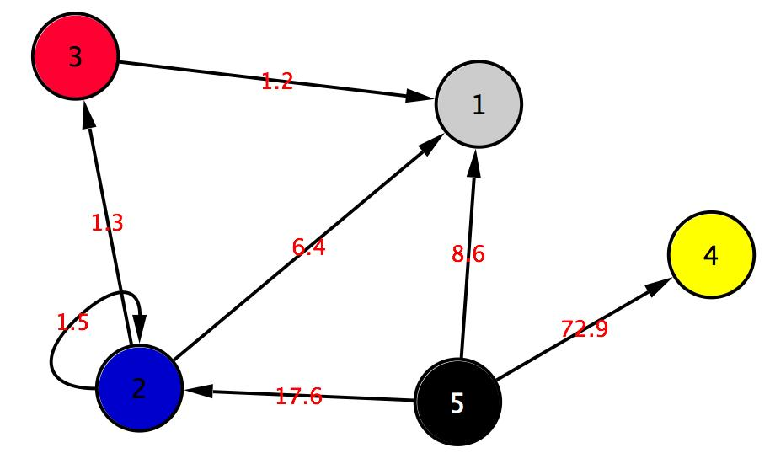
\includegraphics[width=.4\textwidth]{\fignet/VEMmetagraphe.png}
      $$
      
      \bigskip
      \paragraph{Choosing $K$:} penalized 'likelihood'
    \end{tabular}
    & 
    \begin{tabular}{p{.5\textwidth}}
      \includegraphics[width=.4\textwidth]{\fignet/im_EcoliVEM_2}
    \end{tabular}
  \end{tabular}
  
}

%==================================================================
\frame{ \frametitle{Accounting for covariates}

  \paragraph{Same story as network inference:} accounting for available information on nodes ($x_i$) or pairs ($x_{ij}$) may avoid to re-discover the wheel
  
  \bigskip \bigskip \pause
  \paragraph{Including covariates} is often easy (at least formally) adding a regression term:
  $$
  \text{logit}(\Pr\{Y_{ij} = 1 \mid Z_i=k, Z_j=\ell\}) = \alpha_{k\ell} + x_{ij}^\intercal \beta
  $$
  (where $\text{logit}(p) = \log(p/(1-p))$)
  
  \bigskip \pause
  \begin{itemize}
   \item Aims at analysing the structure of the network, that is {\sl not explained} by the covariates ('residual' structure)
%    \item The edges are not exchangeable anymore
   \item Easier to account for edge covariates ($x_{ij}$), than node covariates ($x_i$)
  \end{itemize}
  
  \bigskip \bigskip \pause
  \paragraph{Next: Poisson stochastic blockmodel with covariates:} \refer{MRV10}
  $$
  (Y_{ij} \mid Z_i=k, Z_j=\ell) \sim \Pcal(\exp(\alpha_{k\ell} + x_{ij}^\intercal \beta))
  $$

}

%====================================================================
\frame{ \frametitle{Ecological network (1/2)}

  \begin{tabular}{cc}
    \hspace{-.04\textwidth}
    \begin{tabular}{p{.4\textwidth}}
      \paragraph{Data:} 
      \begin{itemize}
       \item $n = 51$ tree species,
       \item $X_{ij}=$ number of fungal parasites shared by species $i$ and $j$ (\refer{VPD08}).
      \end{itemize}

      \bigskip \bigskip \pause
      \paragraph{Model:}
      $$
      Y_{ij} \sim \Pcal(\lambda_{k\ell}),
      $$
      $\lambda_{k\ell} =$ mean number of common parasites.

      \bigskip \bigskip 
      \paragraph{Results:} ICL selects $K=7$ groups
      that are \emphase{partly related with phylums}. \pause
    \end{tabular}
    & 
    \hspace{-.05\textwidth}
    \begin{tabular}{c}
      {\tiny
        \begin{tabular}{c|ccccccc}
          $\widehat{\lambda}_{q\ell}$ & T1 & T2 & T3 & T4 & T5 & T6 &
          T7 \\ 
          \hline
          T1 & 14.46 & 4.19 & 5.99 & 7.67 & 2.44 & 0.13 & 1.43 \\
          T2 &  & 14.13 & 0.68 & 2.79 & 4.84 & 0.53 & 1.54 \\
          T3 &  &  & 3.19 & 4.10 & 0.66 & 0.02 & 0.69 \\
          T4 &  &  &  & 7.42 & 2.57 & 0.04 & 1.05 \\
          T5 &  &  &  &  & 3.64 & 0.23 & 0.83 \\
          T6 &  &  &  &  &  & 0.04 & 0.06 \\
          T7 &  &  &  &  &  &  & 0.27 \\
          \hline \hline
          $\widehat{\alpha}_q$ & 7.8 & 7.8 & 13.7 & 13.7 & 15.7 & 19.6 &
          21.6  
        \end{tabular}
        }\\ \pause
        
        \bigskip
        $$
        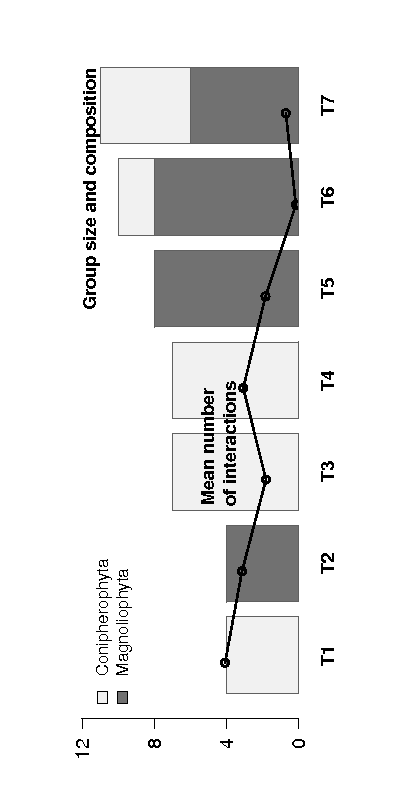
\includegraphics[width=.5\textwidth, trim=150 150 150 150, clip=]{\fignet/MRV10_AoAS_Q7_group}
        $$
    \end{tabular}
  \end{tabular}
  }

%====================================================================
\frame{ \frametitle{Ecological network (2/2)}

  \begin{tabular}{cc}
    \hspace{-.04\textwidth}
    \begin{tabular}{p{.4\textwidth}}
      \paragraph{Accounting for phylogeny:} 
      \begin{itemize}
       \item $x_{ij}=$ taxonimic distance between species $i$ and $j$.
      \end{itemize}

      \bigskip \bigskip \pause
      \paragraph{Model:}
      $$
      X_{ij} \sim \Pcal(\exp(\alpha_{k\ell} + x_{ij}^\intercal \beta)),
      $$
      \ra $\widehat{\beta} = -0.317$ (makes sense !)

      \bigskip \bigskip 
      \paragraph{Results:} ICL selects $K=4$ groups
      that are \emphase{not related with phylums}. \pause
    \end{tabular}
    & 
    \hspace{-.05\textwidth}
    \begin{tabular}{c}
      {\tiny
        \begin{tabular}{c|cccc}
          $\widehat{\lambda}_{q\ell}$ & T'1 & T'2 & T'3 & T'4 \\ 
          \hline
          T'1 & 0.75 & 2.46 & 0.40 & 3.77 \\
          T'2 &  & 4.30 & 0.52 & 8.77 \\ 
          T'3 &  &  & 0.080 & 1.05 \\ 
          T'4 &  &  &  & 14.22 \\
          \hline \hline
          $\widehat{\alpha}_q$ & 17.7 & 21.5 & 23.5 & 37.3 \\
          \hline \hline
          $\widehat{\beta}$ & \multicolumn{4}{c}{-0.317}
        \end{tabular}
        }\\ \pause
      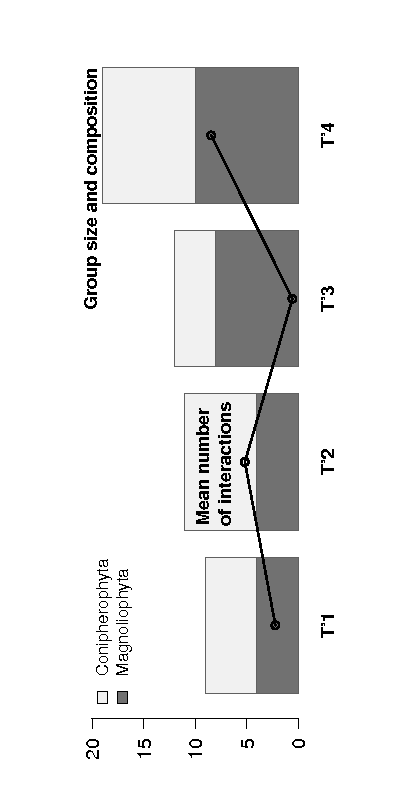
\includegraphics[width=.5\textwidth, trim=150 150 150 150, clip=]{\fignet/MRV10_AoAS_Q4_group}
    \end{tabular}
  \end{tabular}
  }



% %-------------------------------------------------------------------------------
%-------------------------------------------------------------------------------
\section{Network analysis: null models}
%-------------------------------------------------------------------------------
%-------------------------------------------------------------------------------

%------------------------------------------------------------------------------
\frame{ \frametitle{}

}




%-------------------------------------------------------------------------------
%-------------------------------------------------------------------------------
\section{Discussion}
%-------------------------------------------------------------------------------
%-------------------------------------------------------------------------------

%==================================================================
\frame{\frametitle{Network inference}

  \paragraph{Network inference is} 
  \begin{itemize}
   \item Not always a very well-posed problem
   \item A difficult task because of its combinatorial dimension ('a needle in a haystack')
   \item Slightly easier for undirected networks
   \item A highly unsupervised problem (nobody knows the truth, few experimental validations exist)
  \end{itemize}
  
  \bigskip \bigskip \pause
  \begin{tabular}{ll}
    \hspace{-.04\textwidth}
    \begin{tabular}{p{.6\textwidth}}
      \paragraph{Take-home-message} 
      \begin{itemize}
      \item It is not hopeless (although ...)
      \item Graphical models provide a sound mathematical framework 
      \item Reasonably simple tools (R packages) exist 
      \item Accounting for samplign effort and covariates has a dramatic effect on the inferred network
      \item Always ask if the question is a network question \refer{JFS16}
      \end{itemize}
    \end{tabular}
    &
    \pause
    \hspace{-.05\textwidth}
    \begin{tabular}{p{.4\textwidth}}
      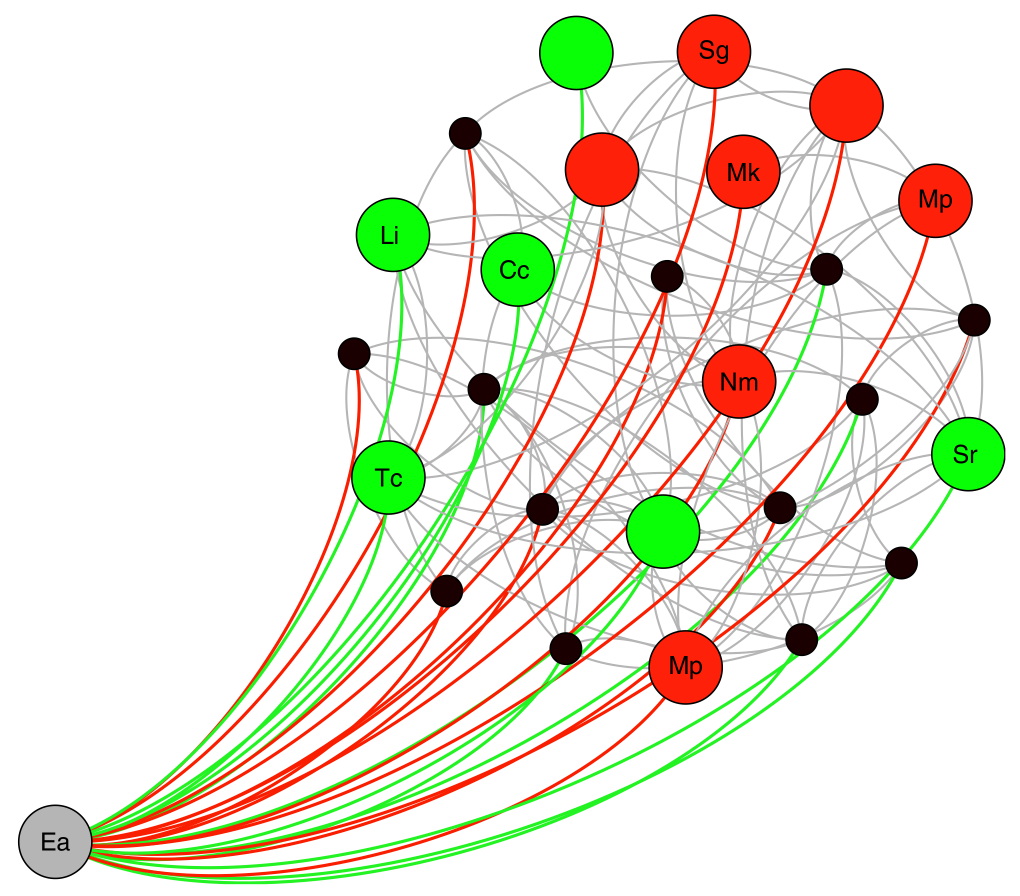
\includegraphics[width=.3\textwidth]{\fignet/JFS16-EnvirMicrobiol-Fig4}
    \end{tabular}
  \end{tabular}

}

%==================================================================
\frame{\frametitle{Network structure}
  
  \paragraph{Statistical models = random graph models.} Can be used to \\~
  \begin{itemize}
    \item exhibit latent structure \\~
    \item correct for expected effects (e.g. covariates) and enhanced unexpected ones
%     \item to serve as (not too) null model to be compared with observation (and to exhibit some {\sl residual} structure)
  \end{itemize}

  \bigskip \bigskip \pause
  \paragraph{Many other ways to analyse a network structure (topology).} \\~
  \begin{itemize}
    \item Global descriptors: density, connectivity, 'nestedness' \\~
    \item Node characteristics: degree distribution, 'edge-betweenness'\\~
    \item Meso-scale descriptors: motifs \\~
  \end{itemize}
  \ra Again: need for a ('null') model to assess the significance of observed values (e.g; configuration model, expected degree model, etc)
    
}


%====================================================================
\backupbegin

%====================================================================
\frame[allowframebreaks]{ \frametitle{References}
  {%\footnotesize
   \tiny
   \bibliography{/home/robin/Biblio/BibGene}
%    \bibliographystyle{/home/robin/LATEX/Biblio/astats}
   \bibliographystyle{alpha}
  }
}


%====================================================================
\appendix 
%-------------------------------------------------------------------------------
%-------------------------------------------------------------------------------
\section*{Appendix}
%-------------------------------------------------------------------------------
%-------------------------------------------------------------------------------

%-------------------------------------------------------------------------------
%-------------------------------------------------------------------------------
\subsection{Graphical models}
%-------------------------------------------------------------------------------

%==================================================================
\frame{\frametitle{Directed graphs = Bayesian networks}

  \paragraph{Definition.} Let $D$ be a {\sl directed acyclic graph} (\emphase{DAG}), the distribution $p$ is said to factorize in $D$ iff
  $$
  p(x_1, \dots x_n) = \prod_{i=1}^n p(x_i \mid x_{pa_D(i)})
  $$
  where $pa_D(i)$ stands for the set of parents of $i$ in $D$.

  \bigskip \pause
  \begin{tabular}{cc}
    \begin{tabular}{c}
    $  \begin{tikzpicture}
  \input{\figeconet/DAG6nodes-positions}
  
  \draw[arrow] (a) to (b);  \draw[arrow] (a) to (c);
  \draw[arrow] (b) to (d);  \draw[arrowbendleft] (b) to (f);
  \draw[arrow] (c) to (d);  \draw[arrow] (d) to (e);
  \draw[arrow] (d) to (f);  
  \end{tikzpicture}
$
    \end{tabular}
    &
    \begin{tabular}{p{.7\textwidth}}
      \begin{eqnarray*}
        pa_D(A) = \emptyset, & & pa_D(D) = \{B, C\}, \qquad \dots  \\
        \\
        p(a, \dots f) & = 
        & p(a) \; p(b \mid a) \; p(c \mid a) \\
        & & p(d \mid b, c) \; p(e \mid d) \\
        & & p(f \mid b, d)
        \end{eqnarray*}
    \end{tabular}
  \end{tabular}
  
  \bigskip
  See \refer{SWA17} for an introduction in ecology
}

%==================================================================
\frame{\frametitle{A simple (interesting) example}

  Consider $D =$
  $$
    \begin{tikzpicture}
  \node[observed] (x) at (0*\edgeunit, 0*\edgeunit) {$X$};
  \node[observed] (y) at (1*\edgeunit, 0*\edgeunit) {$Y$};
  \node[observed] (z) at (2*\edgeunit, 0*\edgeunit) {$Z$};
  
  \draw[arrow] (x) to (y);  \draw[arrow] (y) to (z);
  \end{tikzpicture}

  $$
  $p(x, y, z)$ is faithful to $D$ iff
  $$
  p(x, y, z) = p(x) \; p(y \mid x) \; p(z \mid y) 
  $$ \pause
  But
  \begin{align*}
   p(x) \; p(y \mid x) \; p(z \mid y) 
%    & = p(x) \; \frac{p(x, y)}{p(x)} \; \frac{p(y, z)}{p(y)} \\
%    & = \frac{p(x, y)}{p(y)} \; \frac{p(y, z)}{p(z)} \; p(z) \\
   & = p(x \mid y) \; p(y \mid z) \; p(z) 
  \end{align*}
  so $p$ is also faithful to $D' =$
  $$
    \begin{tikzpicture}
  \node[observed] (x) at (0*\edgeunit, 0*\edgeunit) {$X$};
  \node[observed] (y) at (1*\edgeunit, 0*\edgeunit) {$Y$};
  \node[observed] (z) at (2*\edgeunit, 0*\edgeunit) {$Z$};
  
  \draw[arrow] (z) to (y);  \draw[arrow] (y) to (x);
  \end{tikzpicture}
 
  $$
  \pause and to $D'' =$
  $$
    \begin{tikzpicture}
  \node[observed] (x) at (0*\edgeunit, 0*\edgeunit) {$X$};
  \node[observed] (y) at (1*\edgeunit, 0*\edgeunit) {$Y$};
  \node[observed] (z) at (2*\edgeunit, 0*\edgeunit) {$Z$};
  
  \draw[arrow] (y) to (z);  \draw[arrow] (y) to (x);
  \end{tikzpicture}

  $$
  
  \bigskip \pause
  \paragraph{Conclusions.} 
  \begin{itemize}
   \item $p(x)$ is not enough to retrieve the edge orientations
   \item No causal interpretation (causality not addressed here, see \refer{Pea09,Pea09b})
  \end{itemize}
}
  
%==================================================================
\frame{\frametitle{A nice case: Dynamic 'Bayesian' networks (DBN)}

  \paragraph{Temporal data:} $A_t =$ expression of gene $A$ at time $t$
 
  \bigskip
  \begin{tabular}{p{.48\textwidth}p{.48\textwidth}}
  \paragraph{Genuine graphical model.} A DAG: &
  \paragraph{Usual representation.}  \\ 
  $$
  \renewcommand{\nodesize}{2em}
    \begin{tikzpicture}
  \node[observed] (a1) at (0*\edgeunit, 2.25*\edgeunit) {$A_{t-1}$};
  \node[observed] (b1) at (0*\edgeunit, 1.5*\edgeunit) {$B_{t-1}$};
  \node[observed] (c1) at (0*\edgeunit, .75*\edgeunit) {$C_{t-1}$};
  \node[observed] (d1) at (0*\edgeunit, 0*\edgeunit) {$D_{t-1}$};
  \node[observed] (a2) at (1*\edgeunit, 2.25*\edgeunit) {$A_t$};
  \node[observed] (b2) at (1*\edgeunit, 1.5*\edgeunit) {$B_t$};
  \node[observed] (c2) at (1*\edgeunit, 0.75*\edgeunit) {$C_t$};
  \node[observed] (d2) at (1*\edgeunit, 0*\edgeunit) {$D_t$};
  \node[observed] (a3) at (2*\edgeunit, 2.25*\edgeunit) {$A_{t+1}$};
  \node[observed] (b3) at (2*\edgeunit, 1.5*\edgeunit) {$B_{t+1}$};
  \node[observed] (c3) at (2*\edgeunit, 0.75*\edgeunit) {$C_{t+1}$};
  \node[observed] (d3) at (2*\edgeunit, 0*\edgeunit) {$D_{t+1}$};
  
  \draw[lightarrow] (a1) to (a2);  \draw[lightarrow] (b1) to (b2);
  \draw[lightarrow] (c1) to (c2);  \draw[lightarrow] (d1) to (d2);
  \draw[lightarrow] (a2) to (a3);  \draw[lightarrow] (b2) to (b3);
  \draw[lightarrow] (c2) to (c3);  \draw[lightarrow] (d2) to (d3);

  \draw[arrow] (a1) to (b2);  \draw[arrow] (a1) to (c2);
  \draw[arrow] (b1) to (d2);  
  \draw[arrow] (c1) to (b2);  \draw[arrow] (c1) to (d2);
  \draw[arrow] (d1) to (c2);  \draw[arrow] (d1) to (a2);  

  \draw[arrow] (a2) to (b3);  \draw[arrow] (a2) to (c3);
  \draw[arrow] (b2) to (d3);  
  \draw[arrow] (c2) to (b3);  \draw[arrow] (c2) to (d3);
  \draw[arrow] (d2) to (c3);  \draw[arrow] (d2) to (a3);  
  \end{tikzpicture}

  \renewcommand{\nodesize}{\commonnodesize}
  $$
  &
  $$
  \renewcommand{\nodesize}{2em}
    \begin{tikzpicture}
  \node[observed] (a) at (0*\edgeunit, 1*\edgeunit) {$A$};
  \node[observed] (b) at (1*\edgeunit, 1*\edgeunit) {$B$};
  \node[observed] (c) at (0*\edgeunit, 0*\edgeunit) {$C$};
  \node[observed] (d) at (1*\edgeunit, 0*\edgeunit) {$D$};
  
  \draw[arrow] (a) to (b);  \draw[arrow] (a) to (c);
  \draw[arrow] (b) to (d);  
  \draw[arrow] (c) to (b);  \draw[arrowbendleft] (c) to (d);
  \draw[arrowbendleft] (d) to (c);  \draw[arrow] (d) to (a);  
  
  \end{tikzpicture}

  \renewcommand{\nodesize}{\commonnodesize}
  $$
  (not a DAG)
  \end{tabular}
  
  \paragraph{Simpler reconstruction problem:} 
  Find the parents of each gene $A$, $B$, ... \emphase{independently}
}


%==================================================================
\subsection*{Temporal data}
%==================================================================

%==================================================================
\frame{\frametitle{Temporal data} 

  \paragraph{Data.} $Y_{tj} =$ expression of gene $j$ at time $t$
  $$
  Y_t = (Y_{t1}, \dots, Y_{tp}) = \text{ abundance vector at time $t$}
  $$
  \ra \emphase{Same population} observed along time
  
  \bigskip \bigskip \pause
  \paragraph{A general model.} Markov assumption:
  $$
  p(Y) = p(Y_1) p(Y_2 \mid Y_1) \dots p(Y_n \mid Y_{n-1}) 
  $$
  that is
  $$
  \renewcommand{\nodesize}{2em}
    \begin{tikzpicture}
  \node[observed] (y1)    at (0*\edgeunit, 0*\edgeunit) {$Y_1$};
  \node[nocircle] (y2)       at (1*\edgeunit, 0*\edgeunit) {$\dots$};
  \node[observed] (ytm1)  at (2*\edgeunit, 0*\edgeunit) {$Y_{t-1}$};
  \node[observed] (yt)    at (3*\edgeunit, 0*\edgeunit) {$Y_t$};
  \node[observed] (ytp1)  at (4*\edgeunit, 0*\edgeunit) {$Y_{t+1}$};
  \node[nocircle] (ynm1)     at (5*\edgeunit, 0*\edgeunit) {$\dots$};
  \node[observed] (yn)    at (6*\edgeunit, 0*\edgeunit) {$Y_n$};
  
  \draw[arrow] (y1)   to (y2);  
  \draw[arrow] (y2)   to (ytm1);  
  \draw[arrow] (ytm1) to (yt);  
  \draw[arrow] (yt)   to (ytp1);  
  \draw[arrow] (ytp1) to (ynm1);  
  \draw[arrow] (ynm1) to (yn);  
  \end{tikzpicture}

  \renewcommand{\nodesize}{\commonnodesize}
  $$
  \ra Obviously oriented \\
  \ra Does not say much about gene interactions
  
}

%==================================================================
\frame{\frametitle{A nice case: Dynamic 'Bayesian' networks (DBN)}

  \paragraph{Temporal data:} $A_t =$ expression of gene $A$ at time $t$
  
  \bigskip
  \begin{tabular}{p{.48\textwidth}p{.48\textwidth}}
  \paragraph{Usual representation:} not a DAG &
  \paragraph{Genuine graphical model:} a DAG: \\
  $$
  \renewcommand{\nodesize}{2em}
    \begin{tikzpicture}
  \node[observed] (a) at (0*\edgeunit, 1*\edgeunit) {$A$};
  \node[observed] (b) at (1*\edgeunit, 1*\edgeunit) {$B$};
  \node[observed] (c) at (0*\edgeunit, 0*\edgeunit) {$C$};
  \node[observed] (d) at (1*\edgeunit, 0*\edgeunit) {$D$};
  
  \draw[arrow] (a) to (b);  \draw[arrow] (a) to (c);
  \draw[arrow] (b) to (d);  
  \draw[arrow] (c) to (b);  \draw[arrowbendleft] (c) to (d);
  \draw[arrowbendleft] (d) to (c);  \draw[arrow] (d) to (a);  
  
  \end{tikzpicture}

  \renewcommand{\nodesize}{\commonnodesize}
  $$
  &
  $$
  \renewcommand{\nodesize}{2em}
    \begin{tikzpicture}
  \node[observed] (a1) at (0*\edgeunit, 2.25*\edgeunit) {$A_{t-1}$};
  \node[observed] (b1) at (0*\edgeunit, 1.5*\edgeunit) {$B_{t-1}$};
  \node[observed] (c1) at (0*\edgeunit, .75*\edgeunit) {$C_{t-1}$};
  \node[observed] (d1) at (0*\edgeunit, 0*\edgeunit) {$D_{t-1}$};
  \node[observed] (a2) at (1*\edgeunit, 2.25*\edgeunit) {$A_t$};
  \node[observed] (b2) at (1*\edgeunit, 1.5*\edgeunit) {$B_t$};
  \node[observed] (c2) at (1*\edgeunit, 0.75*\edgeunit) {$C_t$};
  \node[observed] (d2) at (1*\edgeunit, 0*\edgeunit) {$D_t$};
  \node[observed] (a3) at (2*\edgeunit, 2.25*\edgeunit) {$A_{t+1}$};
  \node[observed] (b3) at (2*\edgeunit, 1.5*\edgeunit) {$B_{t+1}$};
  \node[observed] (c3) at (2*\edgeunit, 0.75*\edgeunit) {$C_{t+1}$};
  \node[observed] (d3) at (2*\edgeunit, 0*\edgeunit) {$D_{t+1}$};
  
  \draw[lightarrow] (a1) to (a2);  \draw[lightarrow] (b1) to (b2);
  \draw[lightarrow] (c1) to (c2);  \draw[lightarrow] (d1) to (d2);
  \draw[lightarrow] (a2) to (a3);  \draw[lightarrow] (b2) to (b3);
  \draw[lightarrow] (c2) to (c3);  \draw[lightarrow] (d2) to (d3);

  \draw[arrow] (a1) to (b2);  \draw[arrow] (a1) to (c2);
  \draw[arrow] (b1) to (d2);  
  \draw[arrow] (c1) to (b2);  \draw[arrow] (c1) to (d2);
  \draw[arrow] (d1) to (c2);  \draw[arrow] (d1) to (a2);  

  \draw[arrow] (a2) to (b3);  \draw[arrow] (a2) to (c3);
  \draw[arrow] (b2) to (d3);  
  \draw[arrow] (c2) to (b3);  \draw[arrow] (c2) to (d3);
  \draw[arrow] (d2) to (c3);  \draw[arrow] (d2) to (a3);  
  \end{tikzpicture}

  \renewcommand{\nodesize}{\commonnodesize}
  $$
  \end{tabular}

}

%==================================================================
\frame{\frametitle{Inference}

  \begin{tabular}{p{.48\textwidth}p{.48\textwidth}}
  \paragraph{Multivariate Markov model.} &
  \paragraph{Network to be inferred.}  \\ 
%   $$
%   \renewcommand{\nodesize}{2em}
%     \begin{tikzpicture}
  \node[observed] (a1) at (0*\edgeunit, 2.25*\edgeunit) {$A_{t-1}$};
  \node[observed] (b1) at (0*\edgeunit, 1.5*\edgeunit) {$B_{t-1}$};
  \node[observed] (c1) at (0*\edgeunit, .75*\edgeunit) {$C_{t-1}$};
  \node[observed] (d1) at (0*\edgeunit, 0*\edgeunit) {$D_{t-1}$};
  \node[observed] (a2) at (1*\edgeunit, 2.25*\edgeunit) {$A_t$};
  \node[observed] (b2) at (1*\edgeunit, 1.5*\edgeunit) {$B_t$};
  \node[observed] (c2) at (1*\edgeunit, 0.75*\edgeunit) {$C_t$};
  \node[observed] (d2) at (1*\edgeunit, 0*\edgeunit) {$D_t$};
  \node[observed] (a3) at (2*\edgeunit, 2.25*\edgeunit) {$A_{t+1}$};
  \node[observed] (b3) at (2*\edgeunit, 1.5*\edgeunit) {$B_{t+1}$};
  \node[observed] (c3) at (2*\edgeunit, 0.75*\edgeunit) {$C_{t+1}$};
  \node[observed] (d3) at (2*\edgeunit, 0*\edgeunit) {$D_{t+1}$};
  
  \draw[lightarrow] (a1) to (a2);  \draw[lightarrow] (b1) to (b2);
  \draw[lightarrow] (c1) to (c2);  \draw[lightarrow] (d1) to (d2);
  \draw[lightarrow] (a2) to (a3);  \draw[lightarrow] (b2) to (b3);
  \draw[lightarrow] (c2) to (c3);  \draw[lightarrow] (d2) to (d3);

  \draw[arrow] (a1) to (b2);  \draw[arrow] (a1) to (c2);
  \draw[arrow] (b1) to (d2);  
  \draw[arrow] (c1) to (b2);  \draw[arrow] (c1) to (d2);
  \draw[arrow] (d1) to (c2);  \draw[arrow] (d1) to (a2);  

  \draw[arrow] (a2) to (b3);  \draw[arrow] (a2) to (c3);
  \draw[arrow] (b2) to (d3);  
  \draw[arrow] (c2) to (b3);  \draw[arrow] (c2) to (d3);
  \draw[arrow] (d2) to (c3);  \draw[arrow] (d2) to (a3);  
  \end{tikzpicture}

%   \renewcommand{\nodesize}{\commonnodesize}
%   $$
%   &
%   $$
%   \renewcommand{\nodesize}{2em}
%     \begin{tikzpicture}
  \node[observed] (a) at (0*\edgeunit, 1*\edgeunit) {$A$};
  \node[observed] (b) at (1*\edgeunit, 1*\edgeunit) {$B$};
  \node[observed] (c) at (0*\edgeunit, 0*\edgeunit) {$C$};
  \node[observed] (d) at (1*\edgeunit, 0*\edgeunit) {$D$};
  
  \draw[arrow] (a) to (b);  \draw[arrow] (a) to (c);
  \draw[arrow] (b) to (d);  
  \draw[arrow] (c) to (b);  \draw[arrowbendleft] (c) to (d);
  \draw[arrowbendleft] (d) to (c);  \draw[arrow] (d) to (a);  
  
  \end{tikzpicture}

%   \renewcommand{\nodesize}{\commonnodesize}
%   $$
  \begin{tabular}{c} \includegraphics[trim={175 10 5 5}, scale=.9, clip]{\figeco/SWA17-Nature-Fig1} \end{tabular}
  &
  \begin{tabular}{c} \includegraphics[trim={8 60 180 3}, scale=.9, clip]{\figeco/SWA17-Nature-Fig1} \end{tabular} \\
  Homogeneous along time &  (from \refer{SWA17})
  \end{tabular}
  
  \bigskip \bigskip \pause
  \begin{itemize}
  \item Simpler reconstruction problem: Find the parents of each gene $A$, $B$, ... \emphase{independently}
  \item \emphase{\sl Sparsity} assumption: Each gene has only few parents
  \end{itemize}

}

%==================================================================
\frame{\frametitle{A regression problem}

  \paragraph{A variable selection problem.} To find the parents of gene $k$, write for each time $t$:
  $$
  Y_{t, k} = \sum_j \beta_{jk} Y_{t-1, j} + E_{t, k}
  $$
  and select few $\beta_{jk} \neq 0$ (see e.g. \refer{LBD10})
  
  \bigskip \bigskip \pause
  \paragraph{Extensions.} 
  \begin{itemize}
   \item Presence-absence: logistic regression
   \item Count data: Poisson regression
   \item Other types: generalized linear model (glm)
   \item \pause Most importantly: include covariates
   $$
   Y_{t, k} = \sum_j \beta_{jk} Y_{t-1, j} \; \emphase{+ \sum_h \gamma_{hk} x_{t, h}}  + E_{t, k}
   $$
   where $(x_{t, h}) =$ set of covariates at time $t$.
  \end{itemize}
 
}

%==================================================================
\frame{\frametitle{Variable selection}

  \paragraph{Variable selection:} an old problem, many (many) strategies.

  \bigskip \bigskip \pause
  \paragraph{Inducing sparsity with a penalty.} To get sparse vectors of regression coefficients $\beta_k = (\beta_{jk})_j$, mimimize
  \begin{align*}
    \sum_t \left(Y_{t,k} - \sum_j \beta_{jk} Y_{t-1,j}\right)^2 & + \emphase{\lambda} \sum_{j \neq k} |\beta_{jk}| 
    & & (\text{one gene}) \\
    \text{or} \quad 
    \sum_k \sum_t \left(Y_{t,k} - \sum_j \beta_{jk} Y_{t-1,j}\right)^2 & + \emphase{\lambda} \sum_k \sum_{j \neq k} |\beta_{jk}|
     & & (\text{all genes}) 
  \end{align*}
  
  \bigskip
  'lasso' regression \refer{Tib96,BJM12} = convex problem \\
  \ra Fast solution ({\tt glmnet} R package)
  
  \bigskip \bigskip 
  See \refer{SWA17} for an example with presence-absence data
}



%-------------------------------------------------------------------------------
%-------------------------------------------------------------------------------
\subsection{Random graph models}
%-------------------------------------------------------------------------------

%==================================================================
\frame{ \frametitle{Degree-based models}

  \bigskip 
  \paragraph{Aim:} account for heterogeneous number of neighbors $D_i = \sum_{j \neq i} Y_{ij}$
  
  \bigskip \bigskip \pause
  \hspace{-.04\textwidth}
  \begin{tabular}{p{.45\textwidth}p{.45\textwidth}}  
    \begin{tabular}{p{.45\textwidth}}
      \paragraph{Expected degree distribution (EDD) \refer{ChL02}:} \\
      $$
      p_{ij} := \Pr\{i \sim j\} = d_i d_j / \lambda 
      $$
      $d_i =$ observed degree of node $i$, \\ ~ \\
      $\lambda = \sum_i d_i 
      \quad \Rightarrow \quad 
      \emphase{\Esp D_i = d_i}$ \\ ~ \\
      ($p_{ij}$ may exceed 1...) \\ ~ \\ 
      ~ \\ 
      \onslide+<3>{
      \paragraph{Configuration model} (looks similar but actually different): requires
      $$
      D_i = d_i
      $$
      }
    \end{tabular}
    &
    \hspace{-.05\textwidth}
    \begin{tabular}{p{.45\textwidth}}
      \includegraphics[width=.5\textwidth]{\figeco/florida-EDD-simul.pdf}
    \end{tabular} 
  \end{tabular}

}

%==================================================================
\frame{ \frametitle{EDD for oriented graphs}

  \bigskip
  \paragraph{Degrees:} out-degree $D^+_i = \sum_j Y_{ij}$, in-degree  $D^-_i = \sum_j Y_{ji}$

  \bigskip \bigskip \pause
  \hspace{-.04\textwidth}
  \begin{tabular}{p{.45\textwidth}p{.45\textwidth}}  
    \begin{tabular}{p{.4\textwidth}}
      Connexion probability
      $$
      p_{ij} := \Pr\{i \rightarrow j\} = d^+_i d^-_j / \lambda 
      $$
      \bigskip
      Expected degrees:
      $$
      \Esp D^+_i = d^+_i, 
      \quad 
      \Esp D^-_i = d^-_i
      $$ 
      
      \bigskip
      Only accounts for 'generalists' vs 'specialists' (see top left node) \\
      \bigskip
      \onslide+<3>{
      \paragraph{Again:} similar but different from 'edge rewiring', which imposes
      $$
      D^+_i = d^+_i, \quad D^-_i = d^-_i
      $$}
    \end{tabular}
    &
    \hspace{-.05\textwidth}
    \begin{tabular}{p{.45\textwidth}}
      \includegraphics[width=.5\textwidth]{\figeco/foodweb-baydry-EDD-simul.pdf}
    \end{tabular} 
  \end{tabular}

}

%==================================================================
\frame{ \frametitle{Latent-space models}

  \paragraph{Fact:} observed networks are far from 'random' or 'uniform' (i.e. Erd\"os )
  
  \bigskip \bigskip 
  \paragraph{Rational:} the observed heterogeneity is due to (unobserved) node specificities

  \bigskip \bigskip \pause
  \paragraph{General framework:} latent space models \refer{BJR07,MaR14}
  \begin{itemize}
   \item A latent (= hidden = unobserved) variable $Z_i$ is associated with each node
   \item The connections are independent conditionally on $Z = \{Z_i\}$:
   $$
   \{Y_{ij}\} \text{ indep. } \mid Z:
   \qquad 
   P(Y_{ij} = 1) = \gamma(Z_i, Z_j)
   $$
  \end{itemize}
  
  \bigskip \bigskip \pause
  \paragraph{Exchangeable graphs:} provided that the $Z_i$'s are iid, for any permutation $\sigma$,
  $$
  p(\{Y_{ij}\}) = p(\{Y_{\emphase{\sigma}(i)\emphase{\sigma}(j)}\})
  $$

}

%==================================================================
\frame{ \frametitle{Latent positions}

  \paragraph{Latent position model \refer{HRH02}.} $Z_i \in \Rbb^d$,
  $$
  \log \frac{p_{ij}}{1 - p_{ij}} = \alpha - \|Z_i-Z_j\|
  $$

  \bigskip \pause
  \begin{tabular}{p{.45\textwidth}p{.45\textwidth}}
%     \hspace{-.1\textwidth}
    \begin{tabular}{p{.45\textwidth}}
      Latent positions: \\
      \includegraphics[width=.4\textwidth]{\fignet/LatentPositionModel-Network}
    \end{tabular} 
    &
%     \hspace{-.1\textwidth}
    \begin{tabular}{p{.45\textwidth}}
      Observed data: \\
      \includegraphics[width=.4\textwidth]{\fignet/LatentPositionModel-Adjacency}
    \end{tabular} 
  \end{tabular}
  
  \pause
  \paragraph{Clustering version:} \refer{HRT07}

}

%==================================================================
\frame{ \frametitle{Statistical inference for stochastic blockmodels}

  \paragraph{Exercise:} draw the graphical model of latent variable model for graph
  
  \bigskip
  \begin{tabular}{p{.6\textwidth}p{.4\textwidth}}
    \hspace{-0.04\textwidth}
    \begin{tabular}{p{.5\textwidth}}
      \onslide+<2->{\paragraph{Solution} for $p(Y, Z)$ ~\\}
      \bigskip
      \onslide+<3->{
        \paragraph{Incomplete data model:} $Z$ is not observed \\ ~\\
        \ra Standard statistical inference (e.g. EM algorithm) requires to compute \emphase{$p(Z \mid Y)$} ~\\
        }
      \bigskip
      \onslide+<4->{
        \paragraph{Graph moralization:} the dependency structure of $p(Z \mid Y)$ is (very) intricate \\ ~\\
        \ra Need to resort to Monte-Carlo sampling \refer{NoS01,MSP05} or variational approximations \refer{GoN05,DPR08}
        }
    \end{tabular}
    &
    \begin{tabular}{p{.4\textwidth}}
      \begin{overprint}
        \onslide<2-3>
%           \begin{centering}
            \renewcommand{\nodesize}{1.5em}
              \begin{tikzpicture}
  \node[hidden] (Z1) at (0, \edgeunit) {$Z_1$};
  \node[hidden] (Z2) at (\edgeunit, \edgeunit) {$Z_2$};
  \node[hidden] (Z3) at (0, 0) {$Z_3$};
  \node[hidden] (Z4) at (\edgeunit, 0) {$Z_4$};

  \node[observed] (Y12) at (.5*\edgeunit, 1.75*\edgeunit) {$Y_{12}$};
  \node[observed] (Y13) at (-.75*\edgeunit, .5*\edgeunit) {$Y_{13}$};
  \node[observed] (Y14) at (1.75*\edgeunit, 1.75*\edgeunit) {$Y_{14}$};
  \node[observed] (Y23) at (-.75*\edgeunit, 1.75*\edgeunit) {$Y_{23}$};
  \node[observed] (Y24) at (1.75*\edgeunit, .5*\edgeunit) {$Y_{24}$};
  \node[observed] (Y34) at (.5*\edgeunit, -.75*\edgeunit) {$Y_{34}$};
  
  \draw[arrow] (Z1) to (Y12);  \draw[arrow] (Z2) to (Y12);
  \draw[arrow] (Z1) to (Y13);  \draw[arrow] (Z3) to (Y13);
  \draw[arrow] (Z1) to (Y14);  \draw[arrow] (Z4) to (Y14);
  \draw[arrow] (Z2) to (Y23);  \draw[arrow] (Z3) to (Y23);
  \draw[arrow] (Z2) to (Y24);  \draw[arrow] (Z4) to (Y24);
  \draw[arrow] (Z3) to (Y34);  \draw[arrow] (Z4) to (Y34);
  \end{tikzpicture}

 
%           \end{centering}       
        \onslide<4>
%           \begin{centering}
            \renewcommand{\nodesize}{1.5em}
              \begin{tikzpicture}
  \node[hidden] (Z1) at (0, \edgeunit) {$Z_1$};
  \node[hidden] (Z2) at (\edgeunit, \edgeunit) {$Z_2$};
  \node[hidden] (Z3) at (0, 0) {$Z_3$};
  \node[hidden] (Z4) at (\edgeunit, 0) {$Z_4$};

  \node[observed] (Y12) at (.5*\edgeunit, 1.75*\edgeunit) {$Y_{12}$};
  \node[observed] (Y13) at (-.75*\edgeunit, .5*\edgeunit) {$Y_{13}$};
  \node[observed] (Y14) at (1.75*\edgeunit, 1.75*\edgeunit) {$Y_{14}$};
  \node[observed] (Y23) at (-.75*\edgeunit, 1.75*\edgeunit) {$Y_{23}$};
  \node[observed] (Y24) at (1.75*\edgeunit, .5*\edgeunit) {$Y_{24}$};
  \node[observed] (Y34) at (.5*\edgeunit, -.75*\edgeunit) {$Y_{34}$};
  
  \draw[lightarrow] (Z1) to (Y12);  \draw[lightarrow] (Z2) to (Y12);
  \draw[lightarrow] (Z1) to (Y13);  \draw[lightarrow] (Z3) to (Y13);
  \draw[lightarrow] (Z1) to (Y14);  \draw[lightarrow] (Z4) to (Y14);
  \draw[lightarrow] (Z2) to (Y23);  \draw[lightarrow] (Z3) to (Y23);
  \draw[lightarrow] (Z2) to (Y24);  \draw[lightarrow] (Z4) to (Y24);
  \draw[lightarrow] (Z3) to (Y34);  \draw[lightarrow] (Z4) to (Y34);
  
  \draw[dashededge] (Z1) to (Z2);  \draw[dashededge] (Z1) to (Z3);
  \draw[dashededge] (Z1) to (Z4);  \draw[dashededge] (Z2) to (Z3);
  \draw[dashededge] (Z2) to (Z4);  \draw[dashededge] (Z3) to (Z4);
  \end{tikzpicture}

 
%           \end{centering}       
      \end{overprint}
    \end{tabular} 
  \end{tabular}

}



%====================================================================
\backupend

%====================================================================
%====================================================================
\end{document}
%====================================================================
%====================================================================

%------------------------------------------------------------------------------
\frame{ \frametitle{}

}


  \begin{tabular}{cc}
    \hspace{-.04\textwidth}
    \begin{tabular}{p{.5\textwidth}}
    \end{tabular}
    & 
    \begin{tabular}{p{.5\textwidth}}
    \end{tabular}
  \end{tabular}

